\documentclass[twoside]{book}

% Packages required by doxygen
\usepackage{fixltx2e}
\usepackage{calc}
\usepackage{doxygen}
\usepackage[export]{adjustbox} % also loads graphicx
\usepackage{graphicx}
\usepackage[utf8]{inputenc}
\usepackage{makeidx}
\usepackage{multicol}
\usepackage{multirow}
\PassOptionsToPackage{warn}{textcomp}
\usepackage{textcomp}
\usepackage[nointegrals]{wasysym}
\usepackage[table]{xcolor}

% Font selection
\usepackage[T1]{fontenc}
\usepackage[scaled=.90]{helvet}
\usepackage{courier}
\usepackage{amssymb}
\usepackage{sectsty}
\renewcommand{\familydefault}{\sfdefault}
\allsectionsfont{%
  \fontseries{bc}\selectfont%
  \color{darkgray}%
}
\renewcommand{\DoxyLabelFont}{%
  \fontseries{bc}\selectfont%
  \color{darkgray}%
}
\newcommand{\+}{\discretionary{\mbox{\scriptsize$\hookleftarrow$}}{}{}}

% Page & text layout
\usepackage{geometry}
\geometry{%
  a4paper,%
  top=2.5cm,%
  bottom=2.5cm,%
  left=2.5cm,%
  right=2.5cm%
}
\tolerance=750
\hfuzz=15pt
\hbadness=750
\setlength{\emergencystretch}{15pt}
\setlength{\parindent}{0cm}
\setlength{\parskip}{3ex plus 2ex minus 2ex}
\makeatletter
\renewcommand{\paragraph}{%
  \@startsection{paragraph}{4}{0ex}{-1.0ex}{1.0ex}{%
    \normalfont\normalsize\bfseries\SS@parafont%
  }%
}
\renewcommand{\subparagraph}{%
  \@startsection{subparagraph}{5}{0ex}{-1.0ex}{1.0ex}{%
    \normalfont\normalsize\bfseries\SS@subparafont%
  }%
}
\makeatother

% Headers & footers
\usepackage{fancyhdr}
\pagestyle{fancyplain}
\fancyhead[LE]{\fancyplain{}{\bfseries\thepage}}
\fancyhead[CE]{\fancyplain{}{}}
\fancyhead[RE]{\fancyplain{}{\bfseries\leftmark}}
\fancyhead[LO]{\fancyplain{}{\bfseries\rightmark}}
\fancyhead[CO]{\fancyplain{}{}}
\fancyhead[RO]{\fancyplain{}{\bfseries\thepage}}
\fancyfoot[LE]{\fancyplain{}{}}
\fancyfoot[CE]{\fancyplain{}{}}
\fancyfoot[RE]{\fancyplain{}{\bfseries\scriptsize Generated by Doxygen }}
\fancyfoot[LO]{\fancyplain{}{\bfseries\scriptsize Generated by Doxygen }}
\fancyfoot[CO]{\fancyplain{}{}}
\fancyfoot[RO]{\fancyplain{}{}}
\renewcommand{\footrulewidth}{0.4pt}
\renewcommand{\chaptermark}[1]{%
  \markboth{#1}{}%
}
\renewcommand{\sectionmark}[1]{%
  \markright{\thesection\ #1}%
}

% Indices & bibliography
\usepackage{natbib}
\usepackage[titles]{tocloft}
\setcounter{tocdepth}{3}
\setcounter{secnumdepth}{5}
\makeindex

% Hyperlinks (required, but should be loaded last)
\usepackage{ifpdf}
\ifpdf
  \usepackage[pdftex,pagebackref=true]{hyperref}
\else
  \usepackage[ps2pdf,pagebackref=true]{hyperref}
\fi
\hypersetup{%
  colorlinks=true,%
  linkcolor=blue,%
  citecolor=blue,%
  unicode%
}

% Custom commands
\newcommand{\clearemptydoublepage}{%
  \newpage{\pagestyle{empty}\cleardoublepage}%
}

\usepackage{caption}
\captionsetup{labelsep=space,justification=centering,font={bf},singlelinecheck=off,skip=4pt,position=top}

%===== C O N T E N T S =====

\begin{document}

% Titlepage & ToC
\hypersetup{pageanchor=false,
             bookmarksnumbered=true,
             pdfencoding=unicode
            }
\pagenumbering{roman}
\begin{titlepage}
\vspace*{7cm}
\begin{center}%
{\Large et\+\_\+exploration\+\_\+robot }\\
\vspace*{1cm}
{\large Generated by Doxygen 1.8.11}\\
\end{center}
\end{titlepage}
\clearemptydoublepage
\tableofcontents
\clearemptydoublepage
\pagenumbering{arabic}
\hypersetup{pageanchor=true}

%--- Begin generated contents ---
\chapter{E.\+T. A frontier exploration robot to explore unknown environments}
\label{md__home_srinidhi_catkin_ws_src_et_exploration_robot_README}
\hypertarget{md__home_srinidhi_catkin_ws_src_et_exploration_robot_README}{}
\href{https://travis-ci.com/SrinidhiSreenath/et_exploration_robot}{\tt } \href{https://coveralls.io/github/SrinidhiSreenath/et_exploration_robot?branch=master}{\tt } \href{https://opensource.org/licenses/BSD-3-Clause}{\tt }

\subsection*{Overview}

This project aims to develop the software stack using agile software development process to demonstrate the simulation of a Turtle\+Bot that localizes, maps and autonomously explores the environment when introduced in an unknown environment.

Robotic exploration is a problem that deals with maximizing the information of an area of interest using robots. Exploration using robots is advantageous when humans cannot explore an environment due to inaccessibility or dangerous environmental conditions. One of the booming areas of exploration is space exploration where robotic systems are used to explore extraterrestrial bodies.

Currently, most of the extraterrestrial exploration robots are maintained by national space agencies, but with easier and cheaper access to extraterrestrial space, the demand for robots that explore extraterrestrial terrains is going to increase and create a potential market avenue. By developing exploration robots that map unknown environment, one can cater to industries interested in logging space maps and space mining.

The repository is a R\+OS package implementing a simple exploration with a Turtle\+Bot 2 using frontier based exploration method where it uses frontiers as guidance to explore the unknown space. Frontier based exploration is a technique where frontiers are determined and robot exploration is driven by these frontiers. Frontiers are points on the boundary region between open explored space and unexplored space.

\subsection*{Personnel}

\href{https://www.linkedin.com/in/srinidhisreenath/}{\tt Srinidhi Sreenath}. I am a Mechanical engineer currently pursuing Masters in Robotics at the University of Maryland. My areas of interests include Motion Planning and Decision Making for Self Driving Vehicles.

\subsection*{Dependencies}

This is a R\+OS package which needs
\begin{DoxyItemize}
\item \href{http://wiki.ros.org/kinetic}{\tt R\+OS Kinetic} to be installed on Ubuntu 16.\+04. Installation instructions are outlined \href{http://wiki.ros.org/kinetic/Installation/Ubuntu}{\tt here}.
\item \href{https://www.turtlebot.com/}{\tt Turtlebot} packages are required. Run the following command to install all turtlebot related packages. 
\begin{DoxyCode}
1 sudo apt-get install ros-kinetic-turtlebot*
\end{DoxyCode}

\item \href{http://gazebosim.org/}{\tt Gazebo} version 7.\+0.\+0 or above. Installation instructions can be found \href{http://gazebosim.org/tutorials?cat=guided_b&tut=guided_b1}{\tt here}.
\item Turtle\+Bot \href{http://wiki.ros.org/turtlebot_rviz_launchers}{\tt rviz\+\_\+launchers} and \href{http://wiki.ros.org/move_base}{\tt move\+\_\+base} packages are required. Run the following command to install them. 
\begin{DoxyCode}
1 sudo apt install ros-kinetic-turtlebot-rviz-launchers ros-kinetic-move-base-msgs ros-kinetic-actionlib
       ros-kinetic-actionlib-msgs
\end{DoxyCode}

\end{DoxyItemize}

\subsubsection*{Package dependences}

The following are the package dependies\+:
\begin{DoxyItemize}
\item geometry\+\_\+msgs
\item nav\+\_\+msgs
\item roscpp
\item rospy
\item sensor\+\_\+msgs
\item std\+\_\+msgs
\item visualization\+\_\+msgs
\item tf
\item move\+\_\+base
\item move\+\_\+base\+\_\+msgs
\item actionlib
\end{DoxyItemize}

\subsection*{Build}

In your desired directory, please run the following commands. 
\begin{DoxyCode}
1 mkdir -p ~/catkin\_ws/src
2 cd ~/catkin\_ws/
3 catkin\_make
4 source devel/setup.bash
5 cd src/
6 git clone https://github.com/SrinidhiSreenath/et\_exploration\_robot.git
7 cd ..
8 catkin\_make
\end{DoxyCode}
 \subsection*{Run}

The launch file in the package needs to be launched for simulation. Please run the following commands to launch the desired nodes\+: 
\begin{DoxyCode}
1 cd <path to catkin\_ws>
2 source devel/setup.bash
3 roslaunch et\_exploration\_robot explore.launch
\end{DoxyCode}
 \subsection*{Tests}

To run the goolgle unit tests and rostest integration tests, run the following command in the catkin workspace\+: 
\begin{DoxyCode}
1 catkin\_make run\_tests\_et\_exploration\_robot
\end{DoxyCode}
 To run the unit tests using the launch file, run the following commands in the catkin workspace after all the packages are succesfully built. 
\begin{DoxyCode}
1 cd <path to catkin\_ws>
2 source devel/setup.bash
3 rostest et\_exploration\_robot explorerTests.launch 
\end{DoxyCode}
 \subsection*{Results}

{\itshape To be updated}

\subsection*{Demo}

{\itshape To be updated}

\subsection*{Solo Iterative Process (S\+IP)}

Solo Iterative Process (S\+IP) is used in the development of the project. Test Driven Development appoach is used to comply with the short development cycle. The planning and development of the project is done in three sprints.

\href{https://docs.google.com/spreadsheets/d/1y6k_Kw1-uYTfiacjPWWJsFmW3S48nC0fhaB75R_D93A/edit?usp=sharing}{\tt Product backlog, Iteration backlogs, Work log and Sprint Schedule}.

\href{https://docs.google.com/document/d/1q5BGRm5D0xjOvHy-o9cROjHJibJuXT3Z7A8dWZFaC8w/edit?usp=sharing}{\tt Sprint Planning Notes}

\subsection*{Doxygen Documentation}

\subsection*{Known Issues/ Bugs}

{\itshape To be updated}

\subsection*{Coverage}

{\itshape To be updated} 
\chapter{Hierarchical Index}
\section{Class Hierarchy}
This inheritance list is sorted roughly, but not completely, alphabetically\+:\begin{DoxyCompactList}
\item \contentsline{section}{Explorer}{\pageref{classExplorer}}{}
\item \contentsline{section}{Grid}{\pageref{classGrid}}{}
\item \contentsline{section}{Map}{\pageref{classMap}}{}
\item Test\begin{DoxyCompactList}
\item \contentsline{section}{Explorer\+Test}{\pageref{classExplorerTest}}{}
\item \contentsline{section}{Grid\+Test}{\pageref{classGridTest}}{}
\item \contentsline{section}{Map\+Test}{\pageref{classMapTest}}{}
\end{DoxyCompactList}
\item \contentsline{section}{Test\+Pub}{\pageref{classTestPub}}{}
\end{DoxyCompactList}

\chapter{Class Index}
\section{Class List}
Here are the classes, structs, unions and interfaces with brief descriptions\+:\begin{DoxyCompactList}
\item\contentsline{section}{\hyperlink{classExplorer}{Explorer} \\*Class \hyperlink{classExplorer}{Explorer} }{\pageref{classExplorer}}{}
\item\contentsline{section}{\hyperlink{classExplorerTest}{Explorer\+Test} \\*Class \hyperlink{classExplorerTest}{Explorer\+Test} }{\pageref{classExplorerTest}}{}
\item\contentsline{section}{\hyperlink{classGrid}{Grid} \\*Class \hyperlink{classGrid}{Grid} }{\pageref{classGrid}}{}
\item\contentsline{section}{\hyperlink{classGridTest}{Grid\+Test} \\*Class \hyperlink{classGridTest}{Grid\+Test} }{\pageref{classGridTest}}{}
\item\contentsline{section}{\hyperlink{classMap}{Map} \\*Class \hyperlink{classMap}{Map} }{\pageref{classMap}}{}
\item\contentsline{section}{\hyperlink{classMapTest}{Map\+Test} \\*Class \hyperlink{classMapTest}{Map\+Test} }{\pageref{classMapTest}}{}
\item\contentsline{section}{\hyperlink{classTestPub}{Test\+Pub} \\*Class \hyperlink{classTestPub}{Test\+Pub} }{\pageref{classTestPub}}{}
\end{DoxyCompactList}

\chapter{File Index}
\section{File List}
Here is a list of all documented files with brief descriptions\+:\begin{DoxyCompactList}
\item\contentsline{section}{/home/srinidhi/catkin\+\_\+ws/src/et\+\_\+exploration\+\_\+robot/include/et\+\_\+exploration\+\_\+robot/\hyperlink{explorer_8hpp}{explorer.\+hpp} \\*\hyperlink{classExplorer}{Explorer} class declaration }{\pageref{explorer_8hpp}}{}
\item\contentsline{section}{/home/srinidhi/catkin\+\_\+ws/src/et\+\_\+exploration\+\_\+robot/include/et\+\_\+exploration\+\_\+robot/\hyperlink{grid_8hpp}{grid.\+hpp} \\*\hyperlink{classGrid}{Grid} class declaration }{\pageref{grid_8hpp}}{}
\item\contentsline{section}{/home/srinidhi/catkin\+\_\+ws/src/et\+\_\+exploration\+\_\+robot/include/et\+\_\+exploration\+\_\+robot/\hyperlink{map_8hpp}{map.\+hpp} \\*\hyperlink{classMap}{Map} class declaration }{\pageref{map_8hpp}}{}
\item\contentsline{section}{/home/srinidhi/catkin\+\_\+ws/src/et\+\_\+exploration\+\_\+robot/src/\hyperlink{explorer_8cpp}{explorer.\+cpp} \\*\hyperlink{classExplorer}{Explorer} class method definitions }{\pageref{explorer_8cpp}}{}
\item\contentsline{section}{/home/srinidhi/catkin\+\_\+ws/src/et\+\_\+exploration\+\_\+robot/src/\hyperlink{grid_8cpp}{grid.\+cpp} \\*\hyperlink{classGrid}{Grid} class definitions }{\pageref{grid_8cpp}}{}
\item\contentsline{section}{/home/srinidhi/catkin\+\_\+ws/src/et\+\_\+exploration\+\_\+robot/src/\hyperlink{main_8cpp}{main.\+cpp} \\*Main source file }{\pageref{main_8cpp}}{}
\item\contentsline{section}{/home/srinidhi/catkin\+\_\+ws/src/et\+\_\+exploration\+\_\+robot/src/\hyperlink{map_8cpp}{map.\+cpp} \\*\hyperlink{classMap}{Map} class definition }{\pageref{map_8cpp}}{}
\item\contentsline{section}{/home/srinidhi/catkin\+\_\+ws/src/et\+\_\+exploration\+\_\+robot/test/\hyperlink{explorerTest_8cpp}{explorer\+Test.\+cpp} \\*Rostests for class \hyperlink{classExplorer}{Explorer} }{\pageref{explorerTest_8cpp}}{}
\item\contentsline{section}{/home/srinidhi/catkin\+\_\+ws/src/et\+\_\+exploration\+\_\+robot/test/\hyperlink{gridTest_8cpp}{grid\+Test.\+cpp} \\*Unit tests for class \hyperlink{classGrid}{Grid} }{\pageref{gridTest_8cpp}}{}
\item\contentsline{section}{/home/srinidhi/catkin\+\_\+ws/src/et\+\_\+exploration\+\_\+robot/test/\hyperlink{mainTest_8cpp}{main\+Test.\+cpp} \\*Main file to run all unit tests and rostests }{\pageref{mainTest_8cpp}}{}
\item\contentsline{section}{/home/srinidhi/catkin\+\_\+ws/src/et\+\_\+exploration\+\_\+robot/test/\hyperlink{mapTest_8cpp}{map\+Test.\+cpp} \\*Unit tests for class \hyperlink{classMap}{Map} }{\pageref{mapTest_8cpp}}{}
\end{DoxyCompactList}

\chapter{Class Documentation}
\hypertarget{classExplorer}{}\section{Explorer Class Reference}
\label{classExplorer}\index{Explorer@{Explorer}}


Class \hyperlink{classExplorer}{Explorer}.  




{\ttfamily \#include $<$explorer.\+hpp$>$}

\subsection*{Public Member Functions}
\begin{DoxyCompactItemize}
\item 
\hyperlink{classExplorer_a023c50586b065e67868726a337fb56e0}{Explorer} (const ros\+::\+Node\+Handle \&nh)
\begin{DoxyCompactList}\small\item\em Default constructor for \hyperlink{classExplorer}{Explorer}. Sets up the velocity and marker array publisher topic with R\+OS master and subscribes to occupancy grid map data. \end{DoxyCompactList}\item 
\hyperlink{classExplorer_aa1b0a71e92e003e9162a5ba99d843392}{$\sim$\+Explorer} ()
\begin{DoxyCompactList}\small\item\em Destructor for \hyperlink{classExplorer}{Explorer}. \end{DoxyCompactList}\item 
void \hyperlink{classExplorer_a246ceb49142bbd15bdbdc3b900269294}{explore} ()
\begin{DoxyCompactList}\small\item\em wrapper funtion to intiate and perform all the necessary actions needed for the exploration of the unknown environment by turtlebot \end{DoxyCompactList}\end{DoxyCompactItemize}


\subsection{Detailed Description}
Class \hyperlink{classExplorer}{Explorer}. 

The following class \hyperlink{classExplorer}{Explorer} implements the exploration behavior by determining the frontiers in an unexplored environment and sending navigation goals for a turtlebot. Class \hyperlink{classMap}{Map} is a part of this class. 

\subsection{Constructor \& Destructor Documentation}
\index{Explorer@{Explorer}!Explorer@{Explorer}}
\index{Explorer@{Explorer}!Explorer@{Explorer}}
\subsubsection[{\texorpdfstring{Explorer(const ros\+::\+Node\+Handle \&nh)}{Explorer(const ros::NodeHandle &nh)}}]{\setlength{\rightskip}{0pt plus 5cm}Explorer\+::\+Explorer (
\begin{DoxyParamCaption}
\item[{const ros\+::\+Node\+Handle \&}]{nh}
\end{DoxyParamCaption}
)\hspace{0.3cm}{\ttfamily [explicit]}}\hypertarget{classExplorer_a023c50586b065e67868726a337fb56e0}{}\label{classExplorer_a023c50586b065e67868726a337fb56e0}


Default constructor for \hyperlink{classExplorer}{Explorer}. Sets up the velocity and marker array publisher topic with R\+OS master and subscribes to occupancy grid map data. 


\begin{DoxyParams}{Parameters}
{\em nh} & as R\+OS nodehandle object\\
\hline
\end{DoxyParams}
\begin{DoxyReturn}{Returns}
void 
\end{DoxyReturn}
\index{Explorer@{Explorer}!````~Explorer@{$\sim$\+Explorer}}
\index{````~Explorer@{$\sim$\+Explorer}!Explorer@{Explorer}}
\subsubsection[{\texorpdfstring{$\sim$\+Explorer()}{~Explorer()}}]{\setlength{\rightskip}{0pt plus 5cm}Explorer\+::$\sim$\+Explorer (
\begin{DoxyParamCaption}
{}
\end{DoxyParamCaption}
)}\hypertarget{classExplorer_aa1b0a71e92e003e9162a5ba99d843392}{}\label{classExplorer_aa1b0a71e92e003e9162a5ba99d843392}


Destructor for \hyperlink{classExplorer}{Explorer}. 


\begin{DoxyParams}{Parameters}
{\em none} & \\
\hline
\end{DoxyParams}
\begin{DoxyReturn}{Returns}
void 
\end{DoxyReturn}


\subsection{Member Function Documentation}
\index{Explorer@{Explorer}!explore@{explore}}
\index{explore@{explore}!Explorer@{Explorer}}
\subsubsection[{\texorpdfstring{explore()}{explore()}}]{\setlength{\rightskip}{0pt plus 5cm}void Explorer\+::explore (
\begin{DoxyParamCaption}
{}
\end{DoxyParamCaption}
)}\hypertarget{classExplorer_a246ceb49142bbd15bdbdc3b900269294}{}\label{classExplorer_a246ceb49142bbd15bdbdc3b900269294}


wrapper funtion to intiate and perform all the necessary actions needed for the exploration of the unknown environment by turtlebot 


\begin{DoxyParams}{Parameters}
{\em none} & \\
\hline
\end{DoxyParams}
\begin{DoxyReturn}{Returns}
void 
\end{DoxyReturn}


The documentation for this class was generated from the following files\+:\begin{DoxyCompactItemize}
\item 
/home/srinidhi/catkin\+\_\+ws/src/et\+\_\+exploration\+\_\+robot/include/et\+\_\+exploration\+\_\+robot/\hyperlink{explorer_8hpp}{explorer.\+hpp}\item 
/home/srinidhi/catkin\+\_\+ws/src/et\+\_\+exploration\+\_\+robot/src/\hyperlink{explorer_8cpp}{explorer.\+cpp}\end{DoxyCompactItemize}

\hypertarget{classExplorerTest}{}\section{Explorer\+Test Class Reference}
\label{classExplorerTest}\index{Explorer\+Test@{Explorer\+Test}}


Class \hyperlink{classExplorerTest}{Explorer\+Test}.  




Inheritance diagram for Explorer\+Test\+:
\nopagebreak
\begin{figure}[H]
\begin{center}
\leavevmode
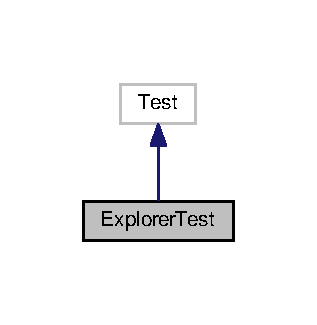
\includegraphics[width=152pt]{classExplorerTest__inherit__graph}
\end{center}
\end{figure}


Collaboration diagram for Explorer\+Test\+:
\nopagebreak
\begin{figure}[H]
\begin{center}
\leavevmode
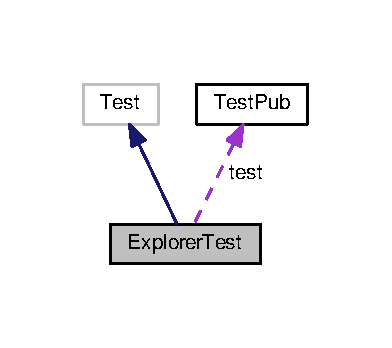
\includegraphics[width=188pt]{classExplorerTest__coll__graph}
\end{center}
\end{figure}
\subsection*{Public Member Functions}
\begin{DoxyCompactItemize}
\item 
void \hyperlink{classExplorerTest_a27a0935c02df6b7bab2bf84e59987a23}{Set\+Up} ()
\begin{DoxyCompactList}\small\item\em Setup function to prepare for each test fixture. \end{DoxyCompactList}\item 
void \hyperlink{classExplorerTest_a8a9ee07a126a1113725f7ed9ea61743f}{Tear\+Down} ()
\begin{DoxyCompactList}\small\item\em Tesrdown function to release any resources allocated in Set\+Up. \end{DoxyCompactList}\end{DoxyCompactItemize}
\subsection*{Protected Attributes}
\begin{DoxyCompactItemize}
\item 
ros\+::\+Node\+Handle \hyperlink{classExplorerTest_a7474ee5196fc4d9017417c3e6511b792}{nh}\hypertarget{classExplorerTest_a7474ee5196fc4d9017417c3e6511b792}{}\label{classExplorerTest_a7474ee5196fc4d9017417c3e6511b792}

\begin{DoxyCompactList}\small\item\em R\+OS Node\+Handle object. \end{DoxyCompactList}\item 
\hyperlink{classTestPub}{Test\+Pub} \hyperlink{classExplorerTest_a5b31f4a2740df7e24805c723b3865d7c}{test}\hypertarget{classExplorerTest_a5b31f4a2740df7e24805c723b3865d7c}{}\label{classExplorerTest_a5b31f4a2740df7e24805c723b3865d7c}

\begin{DoxyCompactList}\small\item\em \hyperlink{classTestPub}{Test\+Pub} object for dummy callbacks. \end{DoxyCompactList}\item 
ros\+::\+Rate \hyperlink{classExplorerTest_a942ab410cdbff899ffbcc96f55777397}{loop\+\_\+rate} = ros\+::\+Rate(10)\hypertarget{classExplorerTest_a942ab410cdbff899ffbcc96f55777397}{}\label{classExplorerTest_a942ab410cdbff899ffbcc96f55777397}

\begin{DoxyCompactList}\small\item\em R\+OS loop rate. \end{DoxyCompactList}\end{DoxyCompactItemize}


\subsection{Detailed Description}
Class \hyperlink{classExplorerTest}{Explorer\+Test}. 

A class to setup and teardown explorer class configurations for test fixtures. 

\subsection{Member Function Documentation}
\index{Explorer\+Test@{Explorer\+Test}!Set\+Up@{Set\+Up}}
\index{Set\+Up@{Set\+Up}!Explorer\+Test@{Explorer\+Test}}
\subsubsection[{\texorpdfstring{Set\+Up()}{SetUp()}}]{\setlength{\rightskip}{0pt plus 5cm}void Explorer\+Test\+::\+Set\+Up (
\begin{DoxyParamCaption}
{}
\end{DoxyParamCaption}
)\hspace{0.3cm}{\ttfamily [inline]}}\hypertarget{classExplorerTest_a27a0935c02df6b7bab2bf84e59987a23}{}\label{classExplorerTest_a27a0935c02df6b7bab2bf84e59987a23}


Setup function to prepare for each test fixture. 


\begin{DoxyParams}{Parameters}
{\em none} & \\
\hline
\end{DoxyParams}
\begin{DoxyReturn}{Returns}
void 
\end{DoxyReturn}
\index{Explorer\+Test@{Explorer\+Test}!Tear\+Down@{Tear\+Down}}
\index{Tear\+Down@{Tear\+Down}!Explorer\+Test@{Explorer\+Test}}
\subsubsection[{\texorpdfstring{Tear\+Down()}{TearDown()}}]{\setlength{\rightskip}{0pt plus 5cm}void Explorer\+Test\+::\+Tear\+Down (
\begin{DoxyParamCaption}
{}
\end{DoxyParamCaption}
)\hspace{0.3cm}{\ttfamily [inline]}}\hypertarget{classExplorerTest_a8a9ee07a126a1113725f7ed9ea61743f}{}\label{classExplorerTest_a8a9ee07a126a1113725f7ed9ea61743f}


Tesrdown function to release any resources allocated in Set\+Up. 


\begin{DoxyParams}{Parameters}
{\em none} & \\
\hline
\end{DoxyParams}
\begin{DoxyReturn}{Returns}
void 
\end{DoxyReturn}


The documentation for this class was generated from the following file\+:\begin{DoxyCompactItemize}
\item 
/home/srinidhi/catkin\+\_\+ws/src/et\+\_\+exploration\+\_\+robot/test/\hyperlink{explorerTest_8cpp}{explorer\+Test.\+cpp}\end{DoxyCompactItemize}

\hypertarget{classGrid}{}\section{Grid Class Reference}
\label{classGrid}\index{Grid@{Grid}}


Class \hyperlink{classGrid}{Grid}.  




{\ttfamily \#include $<$grid.\+hpp$>$}

\subsection*{Public Member Functions}
\begin{DoxyCompactItemize}
\item 
\hyperlink{classGrid_a4ac9ff4f63552b4c61ff90fcb35ad66c}{Grid} ()
\begin{DoxyCompactList}\small\item\em Default constructor for \hyperlink{classGrid}{Grid}. \end{DoxyCompactList}\item 
\hyperlink{classGrid_a3661d0a7f998caaaf8627d7a67072116}{$\sim$\+Grid} ()
\begin{DoxyCompactList}\small\item\em Destructor for \hyperlink{classGrid}{Grid}. \end{DoxyCompactList}\item 
void \hyperlink{classGrid_a82ee6491720390d8f57dc776b7eb4a9c}{set\+Grid\+State} (const uint32\+\_\+t \&height, const uint32\+\_\+t \&width)
\begin{DoxyCompactList}\small\item\em setter function to set the state of the grid cell \end{DoxyCompactList}\item 
std\+::pair$<$ uint32\+\_\+t, uint32\+\_\+t $>$ \hyperlink{classGrid_a4bb7afc469c8d1113912ecc066426c44}{get\+Grid\+State} ()
\begin{DoxyCompactList}\small\item\em getter function to obtain the state of the grid cell \end{DoxyCompactList}\item 
void \hyperlink{classGrid_aba57aa11c35e810c80a47f81e7f8d224}{update\+Probability} (const int8\+\_\+t \&updated\+Probability)
\begin{DoxyCompactList}\small\item\em setter function to set the probablibility of occupancy of the grid cell \end{DoxyCompactList}\item 
int8\+\_\+t \hyperlink{classGrid_a8bdbc0a20221a1a3a0118fb032c21901}{get\+Probability} ()
\begin{DoxyCompactList}\small\item\em getter function to obtain the occupancy probablibility of the grid cell \end{DoxyCompactList}\item 
void \hyperlink{classGrid_a7e1184291fbc7028c0a50391e5f512f0}{set\+Frontier\+Status} (const bool \&status)
\begin{DoxyCompactList}\small\item\em setter function to set the frontier status of the grid cell \end{DoxyCompactList}\item 
bool \hyperlink{classGrid_ae95b1ff42726579e383565945f4044be}{get\+Frontier\+Status} ()
\begin{DoxyCompactList}\small\item\em getter function to obtain the frontier status of the grid cell \end{DoxyCompactList}\item 
void \hyperlink{classGrid_a8660a115b70a5b5e0e7bd4d1f1d3385d}{set\+Cluster\+Number} (const int \&num)
\begin{DoxyCompactList}\small\item\em setter function to set the cluster number of the grid cell \end{DoxyCompactList}\item 
int \hyperlink{classGrid_acd7fc68759fe10c71d0eac828922a1dc}{get\+Cluster\+Number} ()
\begin{DoxyCompactList}\small\item\em getter function to obtain the the cluster number of the grid cell \end{DoxyCompactList}\end{DoxyCompactItemize}


\subsection{Detailed Description}
Class \hyperlink{classGrid}{Grid}. 

The following class \hyperlink{classGrid}{Grid} stores the information of a single grid cell in the occupancy grid map. Information of the grid cell include grid height, width coordinates, occupancy probability, frontier cell status and frontier cluster number. 

\subsection{Constructor \& Destructor Documentation}
\index{Grid@{Grid}!Grid@{Grid}}
\index{Grid@{Grid}!Grid@{Grid}}
\subsubsection[{\texorpdfstring{Grid()}{Grid()}}]{\setlength{\rightskip}{0pt plus 5cm}Grid\+::\+Grid (
\begin{DoxyParamCaption}
{}
\end{DoxyParamCaption}
)}\hypertarget{classGrid_a4ac9ff4f63552b4c61ff90fcb35ad66c}{}\label{classGrid_a4ac9ff4f63552b4c61ff90fcb35ad66c}


Default constructor for \hyperlink{classGrid}{Grid}. 


\begin{DoxyParams}{Parameters}
{\em none} & \\
\hline
\end{DoxyParams}
\begin{DoxyReturn}{Returns}
void 
\end{DoxyReturn}
\index{Grid@{Grid}!````~Grid@{$\sim$\+Grid}}
\index{````~Grid@{$\sim$\+Grid}!Grid@{Grid}}
\subsubsection[{\texorpdfstring{$\sim$\+Grid()}{~Grid()}}]{\setlength{\rightskip}{0pt plus 5cm}Grid\+::$\sim$\+Grid (
\begin{DoxyParamCaption}
{}
\end{DoxyParamCaption}
)}\hypertarget{classGrid_a3661d0a7f998caaaf8627d7a67072116}{}\label{classGrid_a3661d0a7f998caaaf8627d7a67072116}


Destructor for \hyperlink{classGrid}{Grid}. 


\begin{DoxyParams}{Parameters}
{\em none} & \\
\hline
\end{DoxyParams}
\begin{DoxyReturn}{Returns}
void 
\end{DoxyReturn}


\subsection{Member Function Documentation}
\index{Grid@{Grid}!get\+Cluster\+Number@{get\+Cluster\+Number}}
\index{get\+Cluster\+Number@{get\+Cluster\+Number}!Grid@{Grid}}
\subsubsection[{\texorpdfstring{get\+Cluster\+Number()}{getClusterNumber()}}]{\setlength{\rightskip}{0pt plus 5cm}int Grid\+::get\+Cluster\+Number (
\begin{DoxyParamCaption}
{}
\end{DoxyParamCaption}
)}\hypertarget{classGrid_acd7fc68759fe10c71d0eac828922a1dc}{}\label{classGrid_acd7fc68759fe10c71d0eac828922a1dc}


getter function to obtain the the cluster number of the grid cell 


\begin{DoxyParams}{Parameters}
{\em none} & \\
\hline
\end{DoxyParams}
\begin{DoxyReturn}{Returns}
integer value. If the cell is not a frontier cell, then returns -\/1 
\end{DoxyReturn}
\index{Grid@{Grid}!get\+Frontier\+Status@{get\+Frontier\+Status}}
\index{get\+Frontier\+Status@{get\+Frontier\+Status}!Grid@{Grid}}
\subsubsection[{\texorpdfstring{get\+Frontier\+Status()}{getFrontierStatus()}}]{\setlength{\rightskip}{0pt plus 5cm}bool Grid\+::get\+Frontier\+Status (
\begin{DoxyParamCaption}
{}
\end{DoxyParamCaption}
)}\hypertarget{classGrid_ae95b1ff42726579e383565945f4044be}{}\label{classGrid_ae95b1ff42726579e383565945f4044be}


getter function to obtain the frontier status of the grid cell 


\begin{DoxyParams}{Parameters}
{\em none} & \\
\hline
\end{DoxyParams}
\begin{DoxyReturn}{Returns}
boolean value. True if the grid cell is a frontier cell, false otherwise 
\end{DoxyReturn}
\index{Grid@{Grid}!get\+Grid\+State@{get\+Grid\+State}}
\index{get\+Grid\+State@{get\+Grid\+State}!Grid@{Grid}}
\subsubsection[{\texorpdfstring{get\+Grid\+State()}{getGridState()}}]{\setlength{\rightskip}{0pt plus 5cm}std\+::pair$<$ uint32\+\_\+t, uint32\+\_\+t $>$ Grid\+::get\+Grid\+State (
\begin{DoxyParamCaption}
{}
\end{DoxyParamCaption}
)}\hypertarget{classGrid_a4bb7afc469c8d1113912ecc066426c44}{}\label{classGrid_a4bb7afc469c8d1113912ecc066426c44}


getter function to obtain the state of the grid cell 


\begin{DoxyParams}{Parameters}
{\em none} & \\
\hline
\end{DoxyParams}
\begin{DoxyReturn}{Returns}
pair of unsigned integer containing the height and width coordinate of the grid cell 
\end{DoxyReturn}
\index{Grid@{Grid}!get\+Probability@{get\+Probability}}
\index{get\+Probability@{get\+Probability}!Grid@{Grid}}
\subsubsection[{\texorpdfstring{get\+Probability()}{getProbability()}}]{\setlength{\rightskip}{0pt plus 5cm}int8\+\_\+t Grid\+::get\+Probability (
\begin{DoxyParamCaption}
{}
\end{DoxyParamCaption}
)}\hypertarget{classGrid_a8bdbc0a20221a1a3a0118fb032c21901}{}\label{classGrid_a8bdbc0a20221a1a3a0118fb032c21901}


getter function to obtain the occupancy probablibility of the grid cell 


\begin{DoxyParams}{Parameters}
{\em none} & \\
\hline
\end{DoxyParams}
\begin{DoxyReturn}{Returns}
integer denoting the occupancy probablibility 
\end{DoxyReturn}
\index{Grid@{Grid}!set\+Cluster\+Number@{set\+Cluster\+Number}}
\index{set\+Cluster\+Number@{set\+Cluster\+Number}!Grid@{Grid}}
\subsubsection[{\texorpdfstring{set\+Cluster\+Number(const int \&num)}{setClusterNumber(const int &num)}}]{\setlength{\rightskip}{0pt plus 5cm}void Grid\+::set\+Cluster\+Number (
\begin{DoxyParamCaption}
\item[{const int \&}]{num}
\end{DoxyParamCaption}
)}\hypertarget{classGrid_a8660a115b70a5b5e0e7bd4d1f1d3385d}{}\label{classGrid_a8660a115b70a5b5e0e7bd4d1f1d3385d}


setter function to set the cluster number of the grid cell 


\begin{DoxyParams}{Parameters}
{\em num} & is the integer denoting the cluster number\\
\hline
\end{DoxyParams}
\begin{DoxyReturn}{Returns}
void 
\end{DoxyReturn}
\index{Grid@{Grid}!set\+Frontier\+Status@{set\+Frontier\+Status}}
\index{set\+Frontier\+Status@{set\+Frontier\+Status}!Grid@{Grid}}
\subsubsection[{\texorpdfstring{set\+Frontier\+Status(const bool \&status)}{setFrontierStatus(const bool &status)}}]{\setlength{\rightskip}{0pt plus 5cm}void Grid\+::set\+Frontier\+Status (
\begin{DoxyParamCaption}
\item[{const bool \&}]{status}
\end{DoxyParamCaption}
)}\hypertarget{classGrid_a7e1184291fbc7028c0a50391e5f512f0}{}\label{classGrid_a7e1184291fbc7028c0a50391e5f512f0}


setter function to set the frontier status of the grid cell 


\begin{DoxyParams}{Parameters}
{\em status} & is the boolean value denoting whether the grid cell is a frontier cell or not\\
\hline
\end{DoxyParams}
\begin{DoxyReturn}{Returns}
void 
\end{DoxyReturn}
\index{Grid@{Grid}!set\+Grid\+State@{set\+Grid\+State}}
\index{set\+Grid\+State@{set\+Grid\+State}!Grid@{Grid}}
\subsubsection[{\texorpdfstring{set\+Grid\+State(const uint32\+\_\+t \&height, const uint32\+\_\+t \&width)}{setGridState(const uint32_t &height, const uint32_t &width)}}]{\setlength{\rightskip}{0pt plus 5cm}void Grid\+::set\+Grid\+State (
\begin{DoxyParamCaption}
\item[{const uint32\+\_\+t \&}]{height, }
\item[{const uint32\+\_\+t \&}]{width}
\end{DoxyParamCaption}
)}\hypertarget{classGrid_a82ee6491720390d8f57dc776b7eb4a9c}{}\label{classGrid_a82ee6491720390d8f57dc776b7eb4a9c}


setter function to set the state of the grid cell 


\begin{DoxyParams}{Parameters}
{\em height} & is the unsigned integer denoting the height coordinate of the grid cell in the occupancy map \\
\hline
{\em width} & is the unsigned integer denoting the width coordinate of the grid cell in the occupancy map\\
\hline
\end{DoxyParams}
\begin{DoxyReturn}{Returns}
void 
\end{DoxyReturn}
\index{Grid@{Grid}!update\+Probability@{update\+Probability}}
\index{update\+Probability@{update\+Probability}!Grid@{Grid}}
\subsubsection[{\texorpdfstring{update\+Probability(const int8\+\_\+t \&updated\+Probability)}{updateProbability(const int8_t &updatedProbability)}}]{\setlength{\rightskip}{0pt plus 5cm}void Grid\+::update\+Probability (
\begin{DoxyParamCaption}
\item[{const int8\+\_\+t \&}]{updated\+Probability}
\end{DoxyParamCaption}
)}\hypertarget{classGrid_aba57aa11c35e810c80a47f81e7f8d224}{}\label{classGrid_aba57aa11c35e810c80a47f81e7f8d224}


setter function to set the probablibility of occupancy of the grid cell 


\begin{DoxyParams}{Parameters}
{\em updated\+Probability} & is the integer denoting the occupancy probablibility of the grid cell. -\/1 means unexplored, 0 means free and 100 means occupied.\\
\hline
\end{DoxyParams}
\begin{DoxyReturn}{Returns}
void 
\end{DoxyReturn}


The documentation for this class was generated from the following files\+:\begin{DoxyCompactItemize}
\item 
/home/srinidhi/catkin\+\_\+ws/src/et\+\_\+exploration\+\_\+robot/include/et\+\_\+exploration\+\_\+robot/\hyperlink{grid_8hpp}{grid.\+hpp}\item 
/home/srinidhi/catkin\+\_\+ws/src/et\+\_\+exploration\+\_\+robot/src/\hyperlink{grid_8cpp}{grid.\+cpp}\end{DoxyCompactItemize}

\hypertarget{classGridTest}{}\section{Grid\+Test Class Reference}
\label{classGridTest}\index{Grid\+Test@{Grid\+Test}}


Class \hyperlink{classGridTest}{Grid\+Test}.  




Inheritance diagram for Grid\+Test\+:
\nopagebreak
\begin{figure}[H]
\begin{center}
\leavevmode
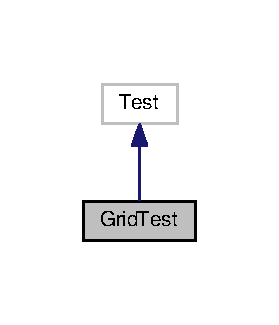
\includegraphics[width=134pt]{classGridTest__inherit__graph}
\end{center}
\end{figure}


Collaboration diagram for Grid\+Test\+:
\nopagebreak
\begin{figure}[H]
\begin{center}
\leavevmode
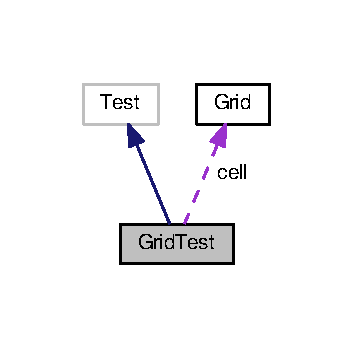
\includegraphics[width=170pt]{classGridTest__coll__graph}
\end{center}
\end{figure}
\subsection*{Public Member Functions}
\begin{DoxyCompactItemize}
\item 
void \hyperlink{classGridTest_accd5f48fb57e88ba96e50a6c4aca470c}{Set\+Up} ()
\begin{DoxyCompactList}\small\item\em Setup function to prepare for each test fixture. \end{DoxyCompactList}\item 
void \hyperlink{classGridTest_ac020afbb1a58be4930e0dc18e859704b}{Tear\+Down} ()
\begin{DoxyCompactList}\small\item\em Tesrdown function to release any resources allocated in Set\+Up. \end{DoxyCompactList}\end{DoxyCompactItemize}
\subsection*{Protected Attributes}
\begin{DoxyCompactItemize}
\item 
\hyperlink{classGrid}{Grid} \hyperlink{classGridTest_abe41b4d65a445d95a553340f81966e5e}{cell}\hypertarget{classGridTest_abe41b4d65a445d95a553340f81966e5e}{}\label{classGridTest_abe41b4d65a445d95a553340f81966e5e}

\begin{DoxyCompactList}\small\item\em Object of class grid. \end{DoxyCompactList}\item 
uint32\+\_\+t \hyperlink{classGridTest_a514f785a55501fbe6009437bda8fe696}{height} = 256\hypertarget{classGridTest_a514f785a55501fbe6009437bda8fe696}{}\label{classGridTest_a514f785a55501fbe6009437bda8fe696}

\begin{DoxyCompactList}\small\item\em height of some desired value \end{DoxyCompactList}\item 
uint32\+\_\+t \hyperlink{classGridTest_a6fe65931252af9de0ff6e9f9699c1a85}{width} = 273\hypertarget{classGridTest_a6fe65931252af9de0ff6e9f9699c1a85}{}\label{classGridTest_a6fe65931252af9de0ff6e9f9699c1a85}

\begin{DoxyCompactList}\small\item\em width of some desired value \end{DoxyCompactList}\item 
int8\+\_\+t \hyperlink{classGridTest_a1bb24df4835b135fd13bef6c40744c8a}{prob} = 7\hypertarget{classGridTest_a1bb24df4835b135fd13bef6c40744c8a}{}\label{classGridTest_a1bb24df4835b135fd13bef6c40744c8a}

\begin{DoxyCompactList}\small\item\em probability of some desired value \end{DoxyCompactList}\item 
int \hyperlink{classGridTest_a79d9337fb35b39b4f49365293947c407}{num} = 91939\hypertarget{classGridTest_a79d9337fb35b39b4f49365293947c407}{}\label{classGridTest_a79d9337fb35b39b4f49365293947c407}

\begin{DoxyCompactList}\small\item\em cluster number of some desired value \end{DoxyCompactList}\end{DoxyCompactItemize}


\subsection{Detailed Description}
Class \hyperlink{classGridTest}{Grid\+Test}. 

A class to setup and teardown grid class configurations for test fixtures. 

\subsection{Member Function Documentation}
\index{Grid\+Test@{Grid\+Test}!Set\+Up@{Set\+Up}}
\index{Set\+Up@{Set\+Up}!Grid\+Test@{Grid\+Test}}
\subsubsection[{\texorpdfstring{Set\+Up()}{SetUp()}}]{\setlength{\rightskip}{0pt plus 5cm}void Grid\+Test\+::\+Set\+Up (
\begin{DoxyParamCaption}
{}
\end{DoxyParamCaption}
)\hspace{0.3cm}{\ttfamily [inline]}}\hypertarget{classGridTest_accd5f48fb57e88ba96e50a6c4aca470c}{}\label{classGridTest_accd5f48fb57e88ba96e50a6c4aca470c}


Setup function to prepare for each test fixture. 


\begin{DoxyParams}{Parameters}
{\em none} & \\
\hline
\end{DoxyParams}
\begin{DoxyReturn}{Returns}
void 
\end{DoxyReturn}
\index{Grid\+Test@{Grid\+Test}!Tear\+Down@{Tear\+Down}}
\index{Tear\+Down@{Tear\+Down}!Grid\+Test@{Grid\+Test}}
\subsubsection[{\texorpdfstring{Tear\+Down()}{TearDown()}}]{\setlength{\rightskip}{0pt plus 5cm}void Grid\+Test\+::\+Tear\+Down (
\begin{DoxyParamCaption}
{}
\end{DoxyParamCaption}
)\hspace{0.3cm}{\ttfamily [inline]}}\hypertarget{classGridTest_ac020afbb1a58be4930e0dc18e859704b}{}\label{classGridTest_ac020afbb1a58be4930e0dc18e859704b}


Tesrdown function to release any resources allocated in Set\+Up. 


\begin{DoxyParams}{Parameters}
{\em none} & \\
\hline
\end{DoxyParams}
\begin{DoxyReturn}{Returns}
void 
\end{DoxyReturn}


The documentation for this class was generated from the following file\+:\begin{DoxyCompactItemize}
\item 
/home/srinidhi/catkin\+\_\+ws/src/et\+\_\+exploration\+\_\+robot/test/\hyperlink{gridTest_8cpp}{grid\+Test.\+cpp}\end{DoxyCompactItemize}

\hypertarget{classMap}{}\section{Map Class Reference}
\label{classMap}\index{Map@{Map}}


Class \hyperlink{classMap}{Map}.  




{\ttfamily \#include $<$map.\+hpp$>$}

\subsection*{Public Member Functions}
\begin{DoxyCompactItemize}
\item 
\hyperlink{classMap_a0f5ad0fd4563497b4214038cbca8b582}{Map} ()
\begin{DoxyCompactList}\small\item\em Default constructor for \hyperlink{classMap}{Map}. \end{DoxyCompactList}\item 
\hyperlink{classMap_aa403fbe09394ccf39747588f5168e3b2}{$\sim$\+Map} ()
\begin{DoxyCompactList}\small\item\em Destructor for \hyperlink{classMap}{Map}. \end{DoxyCompactList}\item 
std\+::vector$<$ uint32\+\_\+t $>$ \hyperlink{classMap_a0407f962dee93f27fd4a4e463cf0f3b1}{get\+Map\+Dimensions} ()
\begin{DoxyCompactList}\small\item\em getter function to obtain the dimesions of the occupancy map i.\+e number of cells in height and width of the map \end{DoxyCompactList}\item 
std\+::pair$<$ float, geometry\+\_\+msgs\+::\+Pose $>$ \hyperlink{classMap_af6dd728dc6d4cb1a7f12968a702781bf}{get\+Map\+Parameters} ()
\begin{DoxyCompactList}\small\item\em getter function to obtain the parameters of the occupancy map i.\+e resolution and origin of the map \end{DoxyCompactList}\item 
std\+::vector$<$ std\+::vector$<$ \hyperlink{classGrid}{Grid} $>$ $>$ \hyperlink{classMap_adc3926804632dcaa2484c552566f7283}{get\+Occupancy\+Grid} ()
\begin{DoxyCompactList}\small\item\em getter function to obtain the occupancy grid map \end{DoxyCompactList}\item 
void \hyperlink{classMap_afc917e8253690d0e3d5b1e31e38ce57d}{initialize} (const nav\+\_\+msgs\+::\+Occupancy\+Grid\+::\+Const\+Ptr \&map)
\begin{DoxyCompactList}\small\item\em function to process occupancy grid map message published and initialize the map. \end{DoxyCompactList}\item 
void \hyperlink{classMap_a666dee0eae4e9a7a2e9870d51459a561}{update\+Occupancy\+Map} (const nav\+\_\+msgs\+::\+Occupancy\+Grid\+::\+Const\+Ptr \&map)
\begin{DoxyCompactList}\small\item\em function to update the occupancy grid map message published in case dimensions or map parameters change \end{DoxyCompactList}\item 
std\+::vector$<$ std\+::vector$<$ std\+::pair$<$ uint32\+\_\+t, uint32\+\_\+t $>$ $>$ $>$ \hyperlink{classMap_a10129fbf19370e76f5bfdceaa32b6f7a}{get\+Frontier\+Clusters} ()
\begin{DoxyCompactList}\small\item\em function that obtain the list of clusters of frontier grid cells. \end{DoxyCompactList}\item 
std\+::vector$<$ std\+::pair$<$ float, float $>$ $>$ \hyperlink{classMap_a00f7910f42acac4789d81ec024bea6f1}{grid\+To\+Cartesian} (const std\+::vector$<$ std\+::pair$<$ uint32\+\_\+t, uint32\+\_\+t $>$$>$ \&frontiers)
\begin{DoxyCompactList}\small\item\em function to convert from grid cell coordinates i.\+e height, width to cartesian coordinates i.\+e x,y in the map \end{DoxyCompactList}\end{DoxyCompactItemize}


\subsection{Detailed Description}
Class \hyperlink{classMap}{Map}. 

The following class \hyperlink{classMap}{Map} stores the occupancy grid map information and determines the frontiers in the map and also performs clustering of the frontiers into different clusters. 

\subsection{Constructor \& Destructor Documentation}
\index{Map@{Map}!Map@{Map}}
\index{Map@{Map}!Map@{Map}}
\subsubsection[{\texorpdfstring{Map()}{Map()}}]{\setlength{\rightskip}{0pt plus 5cm}Map\+::\+Map (
\begin{DoxyParamCaption}
{}
\end{DoxyParamCaption}
)}\hypertarget{classMap_a0f5ad0fd4563497b4214038cbca8b582}{}\label{classMap_a0f5ad0fd4563497b4214038cbca8b582}


Default constructor for \hyperlink{classMap}{Map}. 


\begin{DoxyParams}{Parameters}
{\em none} & \\
\hline
\end{DoxyParams}
\begin{DoxyReturn}{Returns}
void 
\end{DoxyReturn}
\index{Map@{Map}!````~Map@{$\sim$\+Map}}
\index{````~Map@{$\sim$\+Map}!Map@{Map}}
\subsubsection[{\texorpdfstring{$\sim$\+Map()}{~Map()}}]{\setlength{\rightskip}{0pt plus 5cm}Map\+::$\sim$\+Map (
\begin{DoxyParamCaption}
{}
\end{DoxyParamCaption}
)}\hypertarget{classMap_aa403fbe09394ccf39747588f5168e3b2}{}\label{classMap_aa403fbe09394ccf39747588f5168e3b2}


Destructor for \hyperlink{classMap}{Map}. 


\begin{DoxyParams}{Parameters}
{\em none} & \\
\hline
\end{DoxyParams}
\begin{DoxyReturn}{Returns}
void 
\end{DoxyReturn}


\subsection{Member Function Documentation}
\index{Map@{Map}!get\+Frontier\+Clusters@{get\+Frontier\+Clusters}}
\index{get\+Frontier\+Clusters@{get\+Frontier\+Clusters}!Map@{Map}}
\subsubsection[{\texorpdfstring{get\+Frontier\+Clusters()}{getFrontierClusters()}}]{\setlength{\rightskip}{0pt plus 5cm}std\+::vector$<$ std\+::vector$<$ std\+::pair$<$ uint32\+\_\+t, uint32\+\_\+t $>$ $>$ $>$ Map\+::get\+Frontier\+Clusters (
\begin{DoxyParamCaption}
{}
\end{DoxyParamCaption}
)}\hypertarget{classMap_a10129fbf19370e76f5bfdceaa32b6f7a}{}\label{classMap_a10129fbf19370e76f5bfdceaa32b6f7a}


function that obtain the list of clusters of frontier grid cells. 


\begin{DoxyParams}{Parameters}
{\em none} & \\
\hline
\end{DoxyParams}
\begin{DoxyReturn}{Returns}
container of vectors of frontier grid cells as paired unsigned integers. Each vector denotes a cluster. 
\end{DoxyReturn}
\index{Map@{Map}!get\+Map\+Dimensions@{get\+Map\+Dimensions}}
\index{get\+Map\+Dimensions@{get\+Map\+Dimensions}!Map@{Map}}
\subsubsection[{\texorpdfstring{get\+Map\+Dimensions()}{getMapDimensions()}}]{\setlength{\rightskip}{0pt plus 5cm}std\+::vector$<$ uint32\+\_\+t $>$ Map\+::get\+Map\+Dimensions (
\begin{DoxyParamCaption}
{}
\end{DoxyParamCaption}
)}\hypertarget{classMap_a0407f962dee93f27fd4a4e463cf0f3b1}{}\label{classMap_a0407f962dee93f27fd4a4e463cf0f3b1}


getter function to obtain the dimesions of the occupancy map i.\+e number of cells in height and width of the map 


\begin{DoxyParams}{Parameters}
{\em none} & \\
\hline
\end{DoxyParams}
\begin{DoxyReturn}{Returns}
vector of unsigned integer containing the dimensions of the map 
\end{DoxyReturn}
\index{Map@{Map}!get\+Map\+Parameters@{get\+Map\+Parameters}}
\index{get\+Map\+Parameters@{get\+Map\+Parameters}!Map@{Map}}
\subsubsection[{\texorpdfstring{get\+Map\+Parameters()}{getMapParameters()}}]{\setlength{\rightskip}{0pt plus 5cm}std\+::pair$<$ float, geometry\+\_\+msgs\+::\+Pose $>$ Map\+::get\+Map\+Parameters (
\begin{DoxyParamCaption}
{}
\end{DoxyParamCaption}
)}\hypertarget{classMap_af6dd728dc6d4cb1a7f12968a702781bf}{}\label{classMap_af6dd728dc6d4cb1a7f12968a702781bf}


getter function to obtain the parameters of the occupancy map i.\+e resolution and origin of the map 


\begin{DoxyParams}{Parameters}
{\em none} & \\
\hline
\end{DoxyParams}
\begin{DoxyReturn}{Returns}
pair of float and R\+OS message type pose denoting resoltion and origin of map respectively 
\end{DoxyReturn}
\index{Map@{Map}!get\+Occupancy\+Grid@{get\+Occupancy\+Grid}}
\index{get\+Occupancy\+Grid@{get\+Occupancy\+Grid}!Map@{Map}}
\subsubsection[{\texorpdfstring{get\+Occupancy\+Grid()}{getOccupancyGrid()}}]{\setlength{\rightskip}{0pt plus 5cm}std\+::vector$<$ std\+::vector$<$ {\bf Grid} $>$ $>$ Map\+::get\+Occupancy\+Grid (
\begin{DoxyParamCaption}
{}
\end{DoxyParamCaption}
)}\hypertarget{classMap_adc3926804632dcaa2484c552566f7283}{}\label{classMap_adc3926804632dcaa2484c552566f7283}


getter function to obtain the occupancy grid map 


\begin{DoxyParams}{Parameters}
{\em none} & \\
\hline
\end{DoxyParams}
\begin{DoxyReturn}{Returns}
matrix i.\+e vector of vector of grid cells. 
\end{DoxyReturn}
\index{Map@{Map}!grid\+To\+Cartesian@{grid\+To\+Cartesian}}
\index{grid\+To\+Cartesian@{grid\+To\+Cartesian}!Map@{Map}}
\subsubsection[{\texorpdfstring{grid\+To\+Cartesian(const std\+::vector$<$ std\+::pair$<$ uint32\+\_\+t, uint32\+\_\+t $>$$>$ \&frontiers)}{gridToCartesian(const std::vector< std::pair< uint32_t, uint32_t >> &frontiers)}}]{\setlength{\rightskip}{0pt plus 5cm}std\+::vector$<$ std\+::pair$<$ float, float $>$ $>$ Map\+::grid\+To\+Cartesian (
\begin{DoxyParamCaption}
\item[{const std\+::vector$<$ std\+::pair$<$ uint32\+\_\+t, uint32\+\_\+t $>$$>$ \&}]{frontiers}
\end{DoxyParamCaption}
)}\hypertarget{classMap_a00f7910f42acac4789d81ec024bea6f1}{}\label{classMap_a00f7910f42acac4789d81ec024bea6f1}


function to convert from grid cell coordinates i.\+e height, width to cartesian coordinates i.\+e x,y in the map 


\begin{DoxyParams}{Parameters}
{\em vector} & of paired unsigned integer points where each point denotes a frontier in grid cell coordinates\\
\hline
\end{DoxyParams}
\begin{DoxyReturn}{Returns}
vector of paired float points where each point denotes a frontier in cartesian coordinates 
\end{DoxyReturn}
\index{Map@{Map}!initialize@{initialize}}
\index{initialize@{initialize}!Map@{Map}}
\subsubsection[{\texorpdfstring{initialize(const nav\+\_\+msgs\+::\+Occupancy\+Grid\+::\+Const\+Ptr \&map)}{initialize(const nav_msgs::OccupancyGrid::ConstPtr &map)}}]{\setlength{\rightskip}{0pt plus 5cm}void Map\+::initialize (
\begin{DoxyParamCaption}
\item[{const nav\+\_\+msgs\+::\+Occupancy\+Grid\+::\+Const\+Ptr \&}]{map}
\end{DoxyParamCaption}
)}\hypertarget{classMap_afc917e8253690d0e3d5b1e31e38ce57d}{}\label{classMap_afc917e8253690d0e3d5b1e31e38ce57d}


function to process occupancy grid map message published and initialize the map. 


\begin{DoxyParams}{Parameters}
{\em map} & is a boost shared pointer to a message of type nav\+\_\+msgs\+::\+Occupancy\+Grid\\
\hline
\end{DoxyParams}
\begin{DoxyReturn}{Returns}
void 
\end{DoxyReturn}
\index{Map@{Map}!update\+Occupancy\+Map@{update\+Occupancy\+Map}}
\index{update\+Occupancy\+Map@{update\+Occupancy\+Map}!Map@{Map}}
\subsubsection[{\texorpdfstring{update\+Occupancy\+Map(const nav\+\_\+msgs\+::\+Occupancy\+Grid\+::\+Const\+Ptr \&map)}{updateOccupancyMap(const nav_msgs::OccupancyGrid::ConstPtr &map)}}]{\setlength{\rightskip}{0pt plus 5cm}void Map\+::update\+Occupancy\+Map (
\begin{DoxyParamCaption}
\item[{const nav\+\_\+msgs\+::\+Occupancy\+Grid\+::\+Const\+Ptr \&}]{map}
\end{DoxyParamCaption}
)}\hypertarget{classMap_a666dee0eae4e9a7a2e9870d51459a561}{}\label{classMap_a666dee0eae4e9a7a2e9870d51459a561}


function to update the occupancy grid map message published in case dimensions or map parameters change 


\begin{DoxyParams}{Parameters}
{\em map} & is a boost shared pointer to a message of type nav\+\_\+msgs\+::\+Occupancy\+Grid\\
\hline
\end{DoxyParams}
\begin{DoxyReturn}{Returns}
void 
\end{DoxyReturn}


The documentation for this class was generated from the following files\+:\begin{DoxyCompactItemize}
\item 
/home/srinidhi/catkin\+\_\+ws/src/et\+\_\+exploration\+\_\+robot/include/et\+\_\+exploration\+\_\+robot/\hyperlink{map_8hpp}{map.\+hpp}\item 
/home/srinidhi/catkin\+\_\+ws/src/et\+\_\+exploration\+\_\+robot/src/\hyperlink{map_8cpp}{map.\+cpp}\end{DoxyCompactItemize}

\hypertarget{classMapTest}{}\section{Map\+Test Class Reference}
\label{classMapTest}\index{Map\+Test@{Map\+Test}}


Class \hyperlink{classMapTest}{Map\+Test}.  




Inheritance diagram for Map\+Test\+:
\nopagebreak
\begin{figure}[H]
\begin{center}
\leavevmode
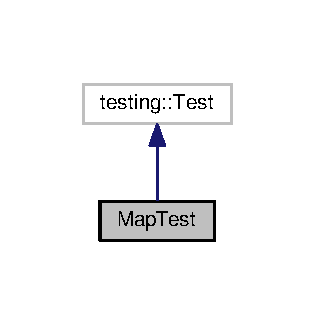
\includegraphics[width=151pt]{classMapTest__inherit__graph}
\end{center}
\end{figure}


Collaboration diagram for Map\+Test\+:
\nopagebreak
\begin{figure}[H]
\begin{center}
\leavevmode
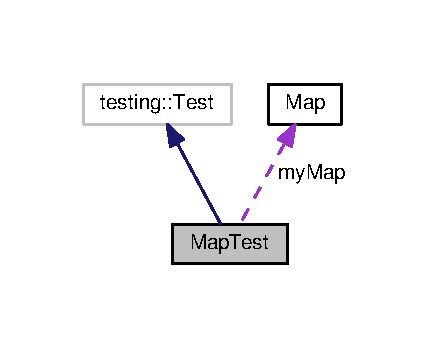
\includegraphics[width=207pt]{classMapTest__coll__graph}
\end{center}
\end{figure}
\subsection*{Public Member Functions}
\begin{DoxyCompactItemize}
\item 
void \hyperlink{classMapTest_a24e2117680abf39f0a8c87c7fffa45fd}{Set\+Up} ()
\begin{DoxyCompactList}\small\item\em Setup function to prepare for each test fixture. Sets a custom map and initializes the map. \end{DoxyCompactList}\item 
void \hyperlink{classMapTest_a4114fafbb5db18eb0052123d062ba18a}{Tear\+Down} ()
\begin{DoxyCompactList}\small\item\em Tesrdown function to release any resources allocated in Set\+Up. \end{DoxyCompactList}\end{DoxyCompactItemize}
\subsection*{Protected Attributes}
\begin{DoxyCompactItemize}
\item 
nav\+\_\+msgs\+::\+Map\+Meta\+Data \hyperlink{classMapTest_a01f5963eaa0d04e9bfa04f4b500251bc}{meta\+Data}
\item 
\hyperlink{classMap}{Map} \hyperlink{classMapTest_ac947eb4207b7fab9c896280a23ab03cd}{my\+Map}\hypertarget{classMapTest_ac947eb4207b7fab9c896280a23ab03cd}{}\label{classMapTest_ac947eb4207b7fab9c896280a23ab03cd}

\begin{DoxyCompactList}\small\item\em Object of class map. \end{DoxyCompactList}\end{DoxyCompactItemize}


\subsection{Detailed Description}
Class \hyperlink{classMapTest}{Map\+Test}. 

A class to setup and teardown map class configurations for test fixtures. 

\subsection{Member Function Documentation}
\index{Map\+Test@{Map\+Test}!Set\+Up@{Set\+Up}}
\index{Set\+Up@{Set\+Up}!Map\+Test@{Map\+Test}}
\subsubsection[{\texorpdfstring{Set\+Up()}{SetUp()}}]{\setlength{\rightskip}{0pt plus 5cm}void Map\+Test\+::\+Set\+Up (
\begin{DoxyParamCaption}
{}
\end{DoxyParamCaption}
)\hspace{0.3cm}{\ttfamily [inline]}}\hypertarget{classMapTest_a24e2117680abf39f0a8c87c7fffa45fd}{}\label{classMapTest_a24e2117680abf39f0a8c87c7fffa45fd}


Setup function to prepare for each test fixture. Sets a custom map and initializes the map. 


\begin{DoxyParams}{Parameters}
{\em none} & \\
\hline
\end{DoxyParams}
\begin{DoxyReturn}{Returns}
void 
\end{DoxyReturn}
\index{Map\+Test@{Map\+Test}!Tear\+Down@{Tear\+Down}}
\index{Tear\+Down@{Tear\+Down}!Map\+Test@{Map\+Test}}
\subsubsection[{\texorpdfstring{Tear\+Down()}{TearDown()}}]{\setlength{\rightskip}{0pt plus 5cm}void Map\+Test\+::\+Tear\+Down (
\begin{DoxyParamCaption}
{}
\end{DoxyParamCaption}
)\hspace{0.3cm}{\ttfamily [inline]}}\hypertarget{classMapTest_a4114fafbb5db18eb0052123d062ba18a}{}\label{classMapTest_a4114fafbb5db18eb0052123d062ba18a}


Tesrdown function to release any resources allocated in Set\+Up. 


\begin{DoxyParams}{Parameters}
{\em none} & \\
\hline
\end{DoxyParams}
\begin{DoxyReturn}{Returns}
void 
\end{DoxyReturn}


\subsection{Member Data Documentation}
\index{Map\+Test@{Map\+Test}!meta\+Data@{meta\+Data}}
\index{meta\+Data@{meta\+Data}!Map\+Test@{Map\+Test}}
\subsubsection[{\texorpdfstring{meta\+Data}{metaData}}]{\setlength{\rightskip}{0pt plus 5cm}nav\+\_\+msgs\+::\+Map\+Meta\+Data Map\+Test\+::meta\+Data\hspace{0.3cm}{\ttfamily [protected]}}\hypertarget{classMapTest_a01f5963eaa0d04e9bfa04f4b500251bc}{}\label{classMapTest_a01f5963eaa0d04e9bfa04f4b500251bc}
R\+OS message of type nav\+\_\+msgs\+::\+Map\+Meta\+Data to define a custom map 

The documentation for this class was generated from the following file\+:\begin{DoxyCompactItemize}
\item 
/home/srinidhi/catkin\+\_\+ws/src/et\+\_\+exploration\+\_\+robot/test/\hyperlink{mapTest_8cpp}{map\+Test.\+cpp}\end{DoxyCompactItemize}

\hypertarget{classTestPub}{}\section{Test\+Pub Class Reference}
\label{classTestPub}\index{Test\+Pub@{Test\+Pub}}


Class \hyperlink{classTestPub}{Test\+Pub}.  


\subsection*{Public Member Functions}
\begin{DoxyCompactItemize}
\item 
\hyperlink{classTestPub_a9b4b3e8a372a68b5497c098e850f6de8}{Test\+Pub} ()
\begin{DoxyCompactList}\small\item\em Default constructor for \hyperlink{classTestPub}{Test\+Pub}. \end{DoxyCompactList}\item 
\hyperlink{classTestPub_a798e9f6a79e8792af0818ca1ac2ae4e4}{$\sim$\+Test\+Pub} ()
\begin{DoxyCompactList}\small\item\em Default destructor for \hyperlink{classTestPub}{Test\+Pub}. \end{DoxyCompactList}\item 
void \hyperlink{classTestPub_a43fe317ee0c36864777704df28aa0823}{vel\+Callback} (const geometry\+\_\+msgs\+::\+Twist\+::\+Const\+Ptr \&msg)
\begin{DoxyCompactList}\small\item\em dummy callback function for subscriber to velocity topic \end{DoxyCompactList}\item 
void \hyperlink{classTestPub_ae1949455b7b7daaf93c265ce9d2b71bc}{marker\+Callback} (const visualization\+\_\+msgs\+::\+Marker\+Array\+::\+Const\+Ptr \&msg)
\begin{DoxyCompactList}\small\item\em dummy callback function for subscriber to markerarray topic \end{DoxyCompactList}\end{DoxyCompactItemize}


\subsection{Detailed Description}
Class \hyperlink{classTestPub}{Test\+Pub}. 

A class to hold dummy callback functions for subscriber callback 

\subsection{Constructor \& Destructor Documentation}
\index{Test\+Pub@{Test\+Pub}!Test\+Pub@{Test\+Pub}}
\index{Test\+Pub@{Test\+Pub}!Test\+Pub@{Test\+Pub}}
\subsubsection[{\texorpdfstring{Test\+Pub()}{TestPub()}}]{\setlength{\rightskip}{0pt plus 5cm}Test\+Pub\+::\+Test\+Pub (
\begin{DoxyParamCaption}
{}
\end{DoxyParamCaption}
)\hspace{0.3cm}{\ttfamily [inline]}}\hypertarget{classTestPub_a9b4b3e8a372a68b5497c098e850f6de8}{}\label{classTestPub_a9b4b3e8a372a68b5497c098e850f6de8}


Default constructor for \hyperlink{classTestPub}{Test\+Pub}. 


\begin{DoxyParams}{Parameters}
{\em none} & \\
\hline
\end{DoxyParams}
\begin{DoxyReturn}{Returns}
void 
\end{DoxyReturn}
\index{Test\+Pub@{Test\+Pub}!````~Test\+Pub@{$\sim$\+Test\+Pub}}
\index{````~Test\+Pub@{$\sim$\+Test\+Pub}!Test\+Pub@{Test\+Pub}}
\subsubsection[{\texorpdfstring{$\sim$\+Test\+Pub()}{~TestPub()}}]{\setlength{\rightskip}{0pt plus 5cm}Test\+Pub\+::$\sim$\+Test\+Pub (
\begin{DoxyParamCaption}
{}
\end{DoxyParamCaption}
)\hspace{0.3cm}{\ttfamily [inline]}}\hypertarget{classTestPub_a798e9f6a79e8792af0818ca1ac2ae4e4}{}\label{classTestPub_a798e9f6a79e8792af0818ca1ac2ae4e4}


Default destructor for \hyperlink{classTestPub}{Test\+Pub}. 


\begin{DoxyParams}{Parameters}
{\em none} & \\
\hline
\end{DoxyParams}
\begin{DoxyReturn}{Returns}
void 
\end{DoxyReturn}


\subsection{Member Function Documentation}
\index{Test\+Pub@{Test\+Pub}!marker\+Callback@{marker\+Callback}}
\index{marker\+Callback@{marker\+Callback}!Test\+Pub@{Test\+Pub}}
\subsubsection[{\texorpdfstring{marker\+Callback(const visualization\+\_\+msgs\+::\+Marker\+Array\+::\+Const\+Ptr \&msg)}{markerCallback(const visualization_msgs::MarkerArray::ConstPtr &msg)}}]{\setlength{\rightskip}{0pt plus 5cm}void Test\+Pub\+::marker\+Callback (
\begin{DoxyParamCaption}
\item[{const visualization\+\_\+msgs\+::\+Marker\+Array\+::\+Const\+Ptr \&}]{msg}
\end{DoxyParamCaption}
)\hspace{0.3cm}{\ttfamily [inline]}}\hypertarget{classTestPub_ae1949455b7b7daaf93c265ce9d2b71bc}{}\label{classTestPub_ae1949455b7b7daaf93c265ce9d2b71bc}


dummy callback function for subscriber to markerarray topic 


\begin{DoxyParams}{Parameters}
{\em msg} & is a boost shared pointer to a message of type visualization\+\_\+msgs\+::\+Marker\+Array\\
\hline
\end{DoxyParams}
\begin{DoxyReturn}{Returns}
void 
\end{DoxyReturn}
\index{Test\+Pub@{Test\+Pub}!vel\+Callback@{vel\+Callback}}
\index{vel\+Callback@{vel\+Callback}!Test\+Pub@{Test\+Pub}}
\subsubsection[{\texorpdfstring{vel\+Callback(const geometry\+\_\+msgs\+::\+Twist\+::\+Const\+Ptr \&msg)}{velCallback(const geometry_msgs::Twist::ConstPtr &msg)}}]{\setlength{\rightskip}{0pt plus 5cm}void Test\+Pub\+::vel\+Callback (
\begin{DoxyParamCaption}
\item[{const geometry\+\_\+msgs\+::\+Twist\+::\+Const\+Ptr \&}]{msg}
\end{DoxyParamCaption}
)\hspace{0.3cm}{\ttfamily [inline]}}\hypertarget{classTestPub_a43fe317ee0c36864777704df28aa0823}{}\label{classTestPub_a43fe317ee0c36864777704df28aa0823}


dummy callback function for subscriber to velocity topic 


\begin{DoxyParams}{Parameters}
{\em msg} & is a boost shared pointer to a message of type geometry\+\_\+msgs\+::\+Twist\\
\hline
\end{DoxyParams}
\begin{DoxyReturn}{Returns}
void 
\end{DoxyReturn}


The documentation for this class was generated from the following file\+:\begin{DoxyCompactItemize}
\item 
/home/srinidhi/catkin\+\_\+ws/src/et\+\_\+exploration\+\_\+robot/test/\hyperlink{explorerTest_8cpp}{explorer\+Test.\+cpp}\end{DoxyCompactItemize}

\chapter{File Documentation}
\hypertarget{explorer_8hpp}{}\section{/home/srinidhi/catkin\+\_\+ws/src/et\+\_\+exploration\+\_\+robot/include/et\+\_\+exploration\+\_\+robot/explorer.hpp File Reference}
\label{explorer_8hpp}\index{/home/srinidhi/catkin\+\_\+ws/src/et\+\_\+exploration\+\_\+robot/include/et\+\_\+exploration\+\_\+robot/explorer.\+hpp@{/home/srinidhi/catkin\+\_\+ws/src/et\+\_\+exploration\+\_\+robot/include/et\+\_\+exploration\+\_\+robot/explorer.\+hpp}}


\hyperlink{classExplorer}{Explorer} class declaration.  


{\ttfamily \#include $<$actionlib/client/simple\+\_\+action\+\_\+client.\+h$>$}\\*
{\ttfamily \#include $<$geometry\+\_\+msgs/\+Pose.\+h$>$}\\*
{\ttfamily \#include $<$geometry\+\_\+msgs/\+Twist.\+h$>$}\\*
{\ttfamily \#include $<$move\+\_\+base\+\_\+msgs/\+Move\+Base\+Action.\+h$>$}\\*
{\ttfamily \#include $<$nav\+\_\+msgs/\+Occupancy\+Grid.\+h$>$}\\*
{\ttfamily \#include $<$ros/ros.\+h$>$}\\*
{\ttfamily \#include $<$tf/transform\+\_\+listener.\+h$>$}\\*
{\ttfamily \#include $<$visualization\+\_\+msgs/\+Marker\+Array.\+h$>$}\\*
{\ttfamily \#include $<$cstdint$>$}\\*
{\ttfamily \#include $<$utility$>$}\\*
{\ttfamily \#include $<$vector$>$}\\*
{\ttfamily \#include \char`\"{}et\+\_\+exploration\+\_\+robot/grid.\+hpp\char`\"{}}\\*
{\ttfamily \#include \char`\"{}et\+\_\+exploration\+\_\+robot/map.\+hpp\char`\"{}}\\*
Include dependency graph for explorer.\+hpp\+:
\nopagebreak
\begin{figure}[H]
\begin{center}
\leavevmode
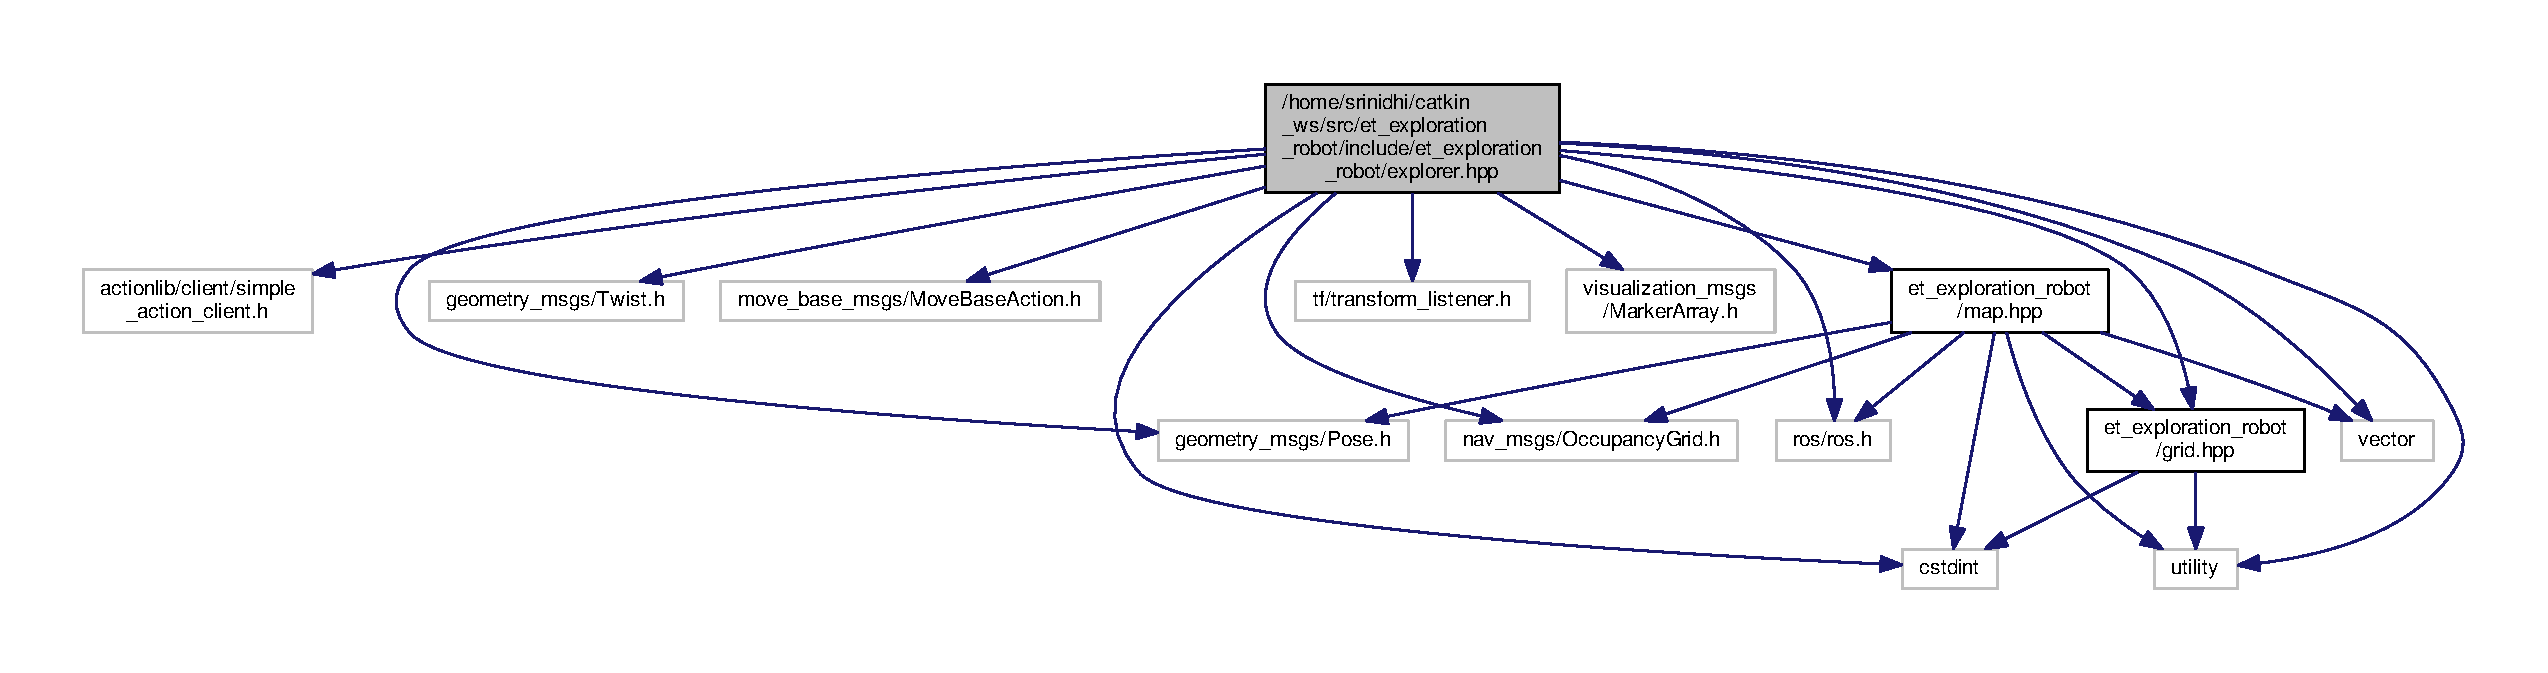
\includegraphics[width=350pt]{explorer_8hpp__incl}
\end{center}
\end{figure}
This graph shows which files directly or indirectly include this file\+:
\nopagebreak
\begin{figure}[H]
\begin{center}
\leavevmode
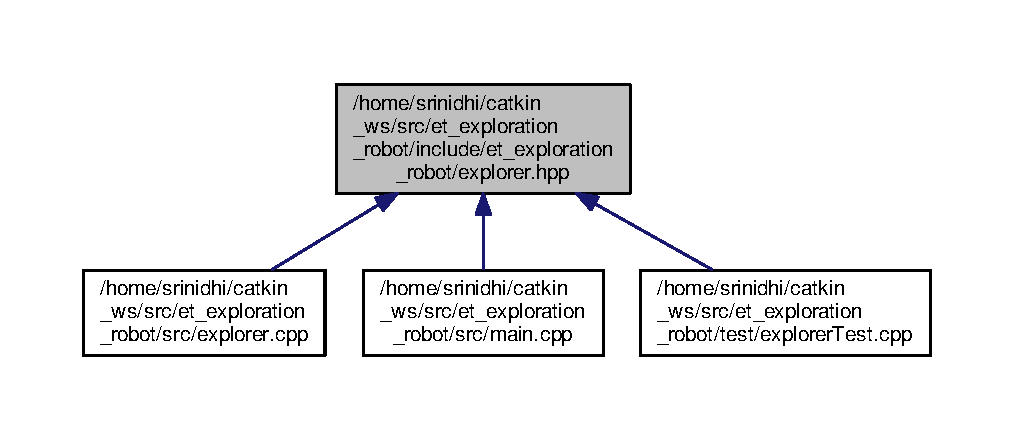
\includegraphics[width=350pt]{explorer_8hpp__dep__incl}
\end{center}
\end{figure}
\subsection*{Classes}
\begin{DoxyCompactItemize}
\item 
class \hyperlink{classExplorer}{Explorer}
\begin{DoxyCompactList}\small\item\em Class \hyperlink{classExplorer}{Explorer}. \end{DoxyCompactList}\end{DoxyCompactItemize}
\subsection*{Typedefs}
\begin{DoxyCompactItemize}
\item 
typedef actionlib\+::\+Simple\+Action\+Client$<$ move\+\_\+base\+\_\+msgs\+::\+Move\+Base\+Action $>$ {\bfseries Move\+Base\+Client}\hypertarget{explorer_8hpp_a21e20cc0b6656ae897b3cbb969b93241}{}\label{explorer_8hpp_a21e20cc0b6656ae897b3cbb969b93241}

\end{DoxyCompactItemize}


\subsection{Detailed Description}
\hyperlink{classExplorer}{Explorer} class declaration. 

\begin{DoxyAuthor}{Author}
Srinidhi Sreenath (Srinidhi\+Sreenath) 
\end{DoxyAuthor}
\begin{DoxyDate}{Date}
12/15/2018 
\end{DoxyDate}
\begin{DoxyVersion}{Version}
1.\+0
\end{DoxyVersion}
\hypertarget{mapTest_8cpp_DESCRIPTION}{}\subsection{D\+E\+S\+C\+R\+I\+P\+T\+I\+ON}\label{mapTest_8cpp_DESCRIPTION}
Header file for class \hyperlink{classExplorer}{Explorer} which implements the exploration behavior for a turtlebot in an unknown environment. 
\hypertarget{grid_8hpp}{}\section{/home/srinidhi/catkin\+\_\+ws/src/et\+\_\+exploration\+\_\+robot/include/et\+\_\+exploration\+\_\+robot/grid.hpp File Reference}
\label{grid_8hpp}\index{/home/srinidhi/catkin\+\_\+ws/src/et\+\_\+exploration\+\_\+robot/include/et\+\_\+exploration\+\_\+robot/grid.\+hpp@{/home/srinidhi/catkin\+\_\+ws/src/et\+\_\+exploration\+\_\+robot/include/et\+\_\+exploration\+\_\+robot/grid.\+hpp}}


\hyperlink{classGrid}{Grid} class declaration.  


{\ttfamily \#include $<$cstdint$>$}\\*
{\ttfamily \#include $<$utility$>$}\\*
Include dependency graph for grid.\+hpp\+:
\nopagebreak
\begin{figure}[H]
\begin{center}
\leavevmode
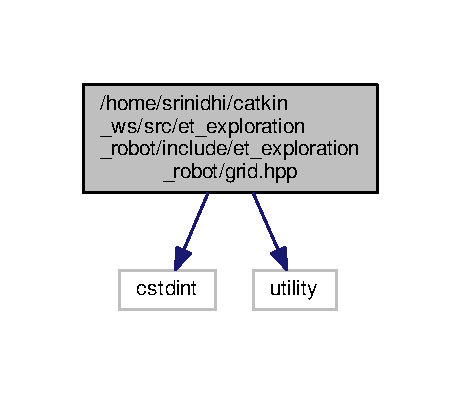
\includegraphics[width=221pt]{grid_8hpp__incl}
\end{center}
\end{figure}
This graph shows which files directly or indirectly include this file\+:
\nopagebreak
\begin{figure}[H]
\begin{center}
\leavevmode
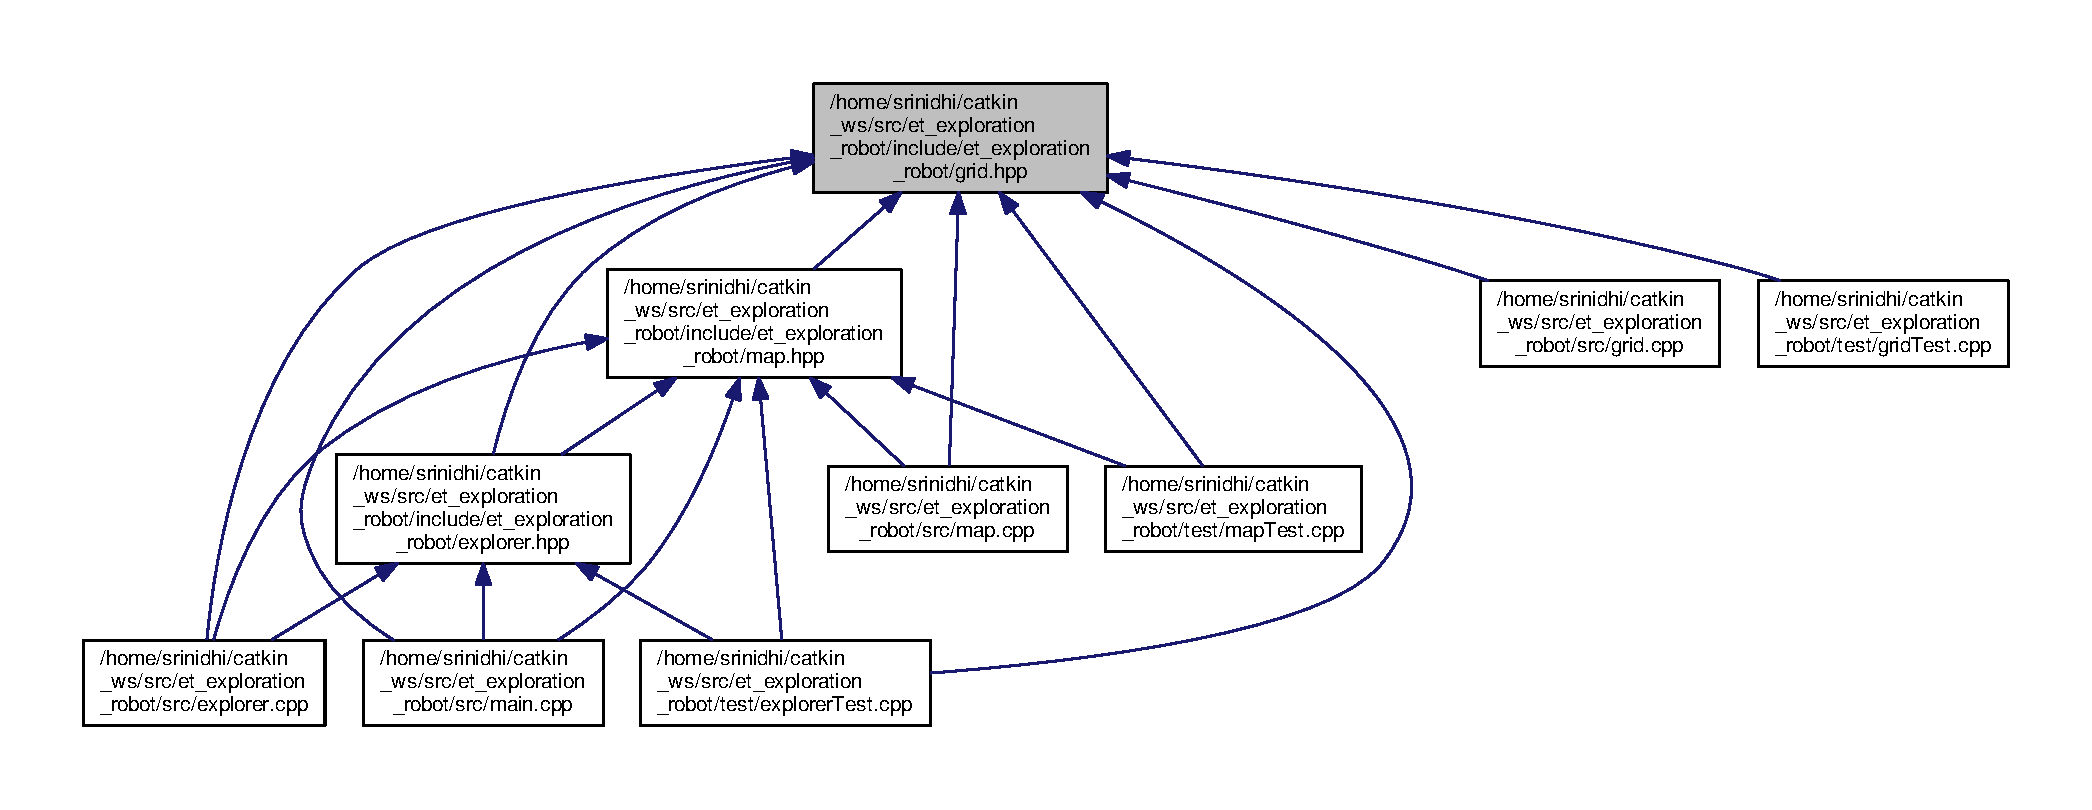
\includegraphics[width=350pt]{grid_8hpp__dep__incl}
\end{center}
\end{figure}
\subsection*{Classes}
\begin{DoxyCompactItemize}
\item 
class \hyperlink{classGrid}{Grid}
\begin{DoxyCompactList}\small\item\em Class \hyperlink{classGrid}{Grid}. \end{DoxyCompactList}\end{DoxyCompactItemize}


\subsection{Detailed Description}
\hyperlink{classGrid}{Grid} class declaration. 

\begin{DoxyAuthor}{Author}
Srinidhi Sreenath (Srinidhi\+Sreenath) 
\end{DoxyAuthor}
\begin{DoxyDate}{Date}
12/15/2018 
\end{DoxyDate}
\begin{DoxyVersion}{Version}
1.\+0
\end{DoxyVersion}
\hypertarget{mapTest_8cpp_DESCRIPTION}{}\subsection{D\+E\+S\+C\+R\+I\+P\+T\+I\+ON}\label{mapTest_8cpp_DESCRIPTION}
Header file for class \hyperlink{classGrid}{Grid} which stores information of a single grid cell in the occupancy grid map. 
\hypertarget{map_8hpp}{}\section{/home/srinidhi/catkin\+\_\+ws/src/et\+\_\+exploration\+\_\+robot/include/et\+\_\+exploration\+\_\+robot/map.hpp File Reference}
\label{map_8hpp}\index{/home/srinidhi/catkin\+\_\+ws/src/et\+\_\+exploration\+\_\+robot/include/et\+\_\+exploration\+\_\+robot/map.\+hpp@{/home/srinidhi/catkin\+\_\+ws/src/et\+\_\+exploration\+\_\+robot/include/et\+\_\+exploration\+\_\+robot/map.\+hpp}}


\hyperlink{classMap}{Map} class declaration.  


{\ttfamily \#include $<$geometry\+\_\+msgs/\+Pose.\+h$>$}\\*
{\ttfamily \#include $<$nav\+\_\+msgs/\+Occupancy\+Grid.\+h$>$}\\*
{\ttfamily \#include $<$ros/ros.\+h$>$}\\*
{\ttfamily \#include $<$cstdint$>$}\\*
{\ttfamily \#include $<$utility$>$}\\*
{\ttfamily \#include $<$vector$>$}\\*
{\ttfamily \#include \char`\"{}et\+\_\+exploration\+\_\+robot/grid.\+hpp\char`\"{}}\\*
Include dependency graph for map.\+hpp\+:
\nopagebreak
\begin{figure}[H]
\begin{center}
\leavevmode
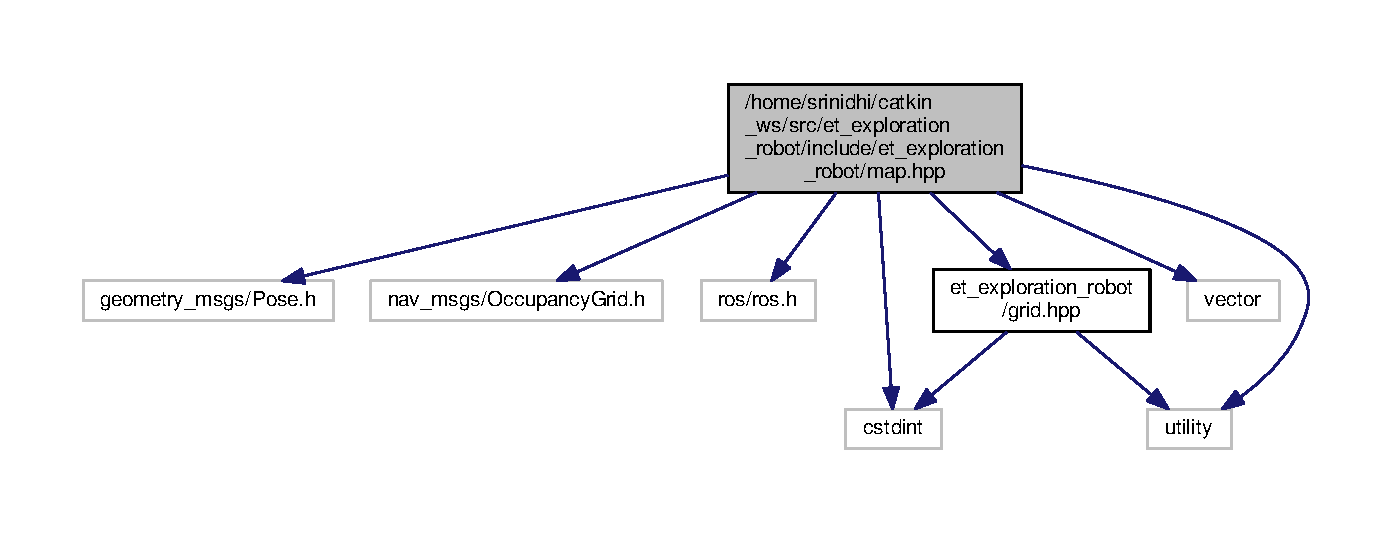
\includegraphics[width=350pt]{map_8hpp__incl}
\end{center}
\end{figure}
This graph shows which files directly or indirectly include this file\+:
\nopagebreak
\begin{figure}[H]
\begin{center}
\leavevmode
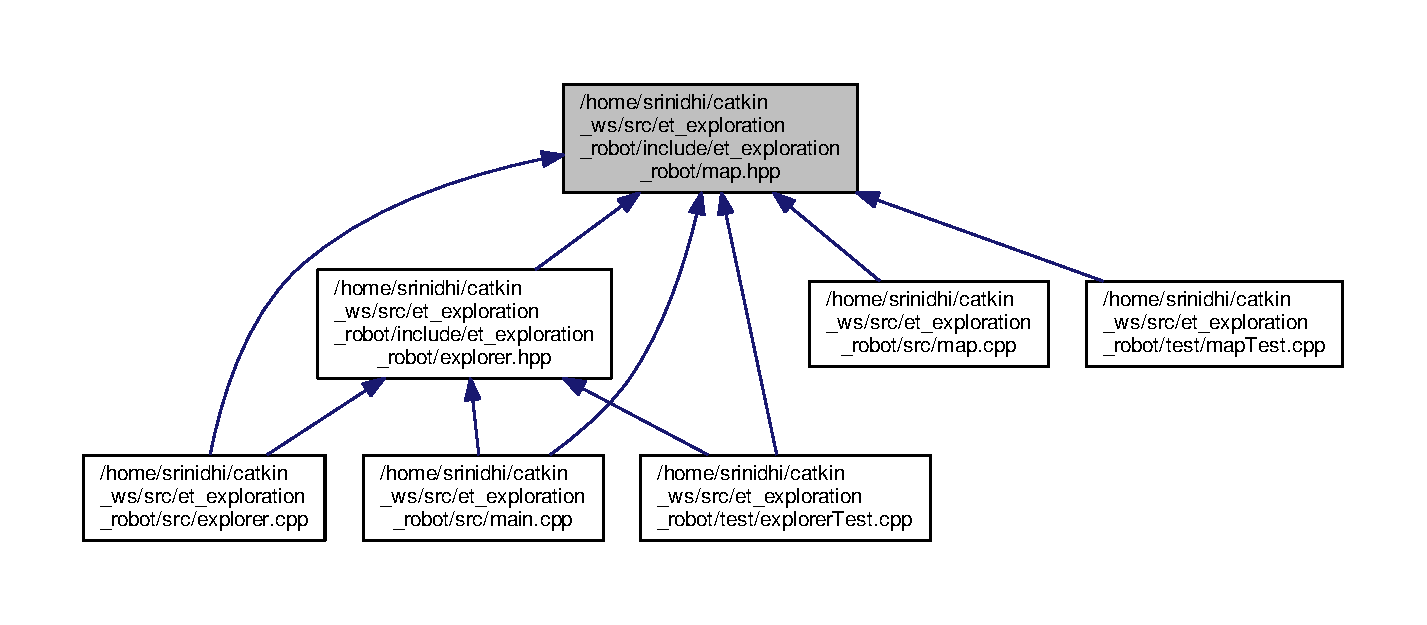
\includegraphics[width=350pt]{map_8hpp__dep__incl}
\end{center}
\end{figure}
\subsection*{Classes}
\begin{DoxyCompactItemize}
\item 
class \hyperlink{classMap}{Map}
\begin{DoxyCompactList}\small\item\em Class \hyperlink{classMap}{Map}. \end{DoxyCompactList}\end{DoxyCompactItemize}


\subsection{Detailed Description}
\hyperlink{classMap}{Map} class declaration. 

\begin{DoxyAuthor}{Author}
Srinidhi Sreenath (Srinidhi\+Sreenath) 
\end{DoxyAuthor}
\begin{DoxyDate}{Date}
12/15/2018 
\end{DoxyDate}
\begin{DoxyVersion}{Version}
1.\+0
\end{DoxyVersion}
\hypertarget{mapTest_8cpp_DESCRIPTION}{}\subsection{D\+E\+S\+C\+R\+I\+P\+T\+I\+ON}\label{mapTest_8cpp_DESCRIPTION}
Header file for class \hyperlink{classMap}{Map} which stores the occupancy grid map information and is used to determine the frontiers in the occupancy grid map. 
\hypertarget{explorer_8cpp}{}\section{/home/srinidhi/catkin\+\_\+ws/src/et\+\_\+exploration\+\_\+robot/src/explorer.cpp File Reference}
\label{explorer_8cpp}\index{/home/srinidhi/catkin\+\_\+ws/src/et\+\_\+exploration\+\_\+robot/src/explorer.\+cpp@{/home/srinidhi/catkin\+\_\+ws/src/et\+\_\+exploration\+\_\+robot/src/explorer.\+cpp}}


\hyperlink{classExplorer}{Explorer} class method definitions.  


{\ttfamily \#include $<$actionlib/client/simple\+\_\+action\+\_\+client.\+h$>$}\\*
{\ttfamily \#include $<$geometry\+\_\+msgs/\+Pose.\+h$>$}\\*
{\ttfamily \#include $<$move\+\_\+base\+\_\+msgs/\+Move\+Base\+Action.\+h$>$}\\*
{\ttfamily \#include $<$nav\+\_\+msgs/\+Occupancy\+Grid.\+h$>$}\\*
{\ttfamily \#include $<$ros/ros.\+h$>$}\\*
{\ttfamily \#include $<$cmath$>$}\\*
{\ttfamily \#include $<$cstdint$>$}\\*
{\ttfamily \#include $<$limits$>$}\\*
{\ttfamily \#include $<$utility$>$}\\*
{\ttfamily \#include $<$vector$>$}\\*
{\ttfamily \#include \char`\"{}et\+\_\+exploration\+\_\+robot/explorer.\+hpp\char`\"{}}\\*
{\ttfamily \#include \char`\"{}et\+\_\+exploration\+\_\+robot/grid.\+hpp\char`\"{}}\\*
{\ttfamily \#include \char`\"{}et\+\_\+exploration\+\_\+robot/map.\+hpp\char`\"{}}\\*
Include dependency graph for explorer.\+cpp\+:
\nopagebreak
\begin{figure}[H]
\begin{center}
\leavevmode
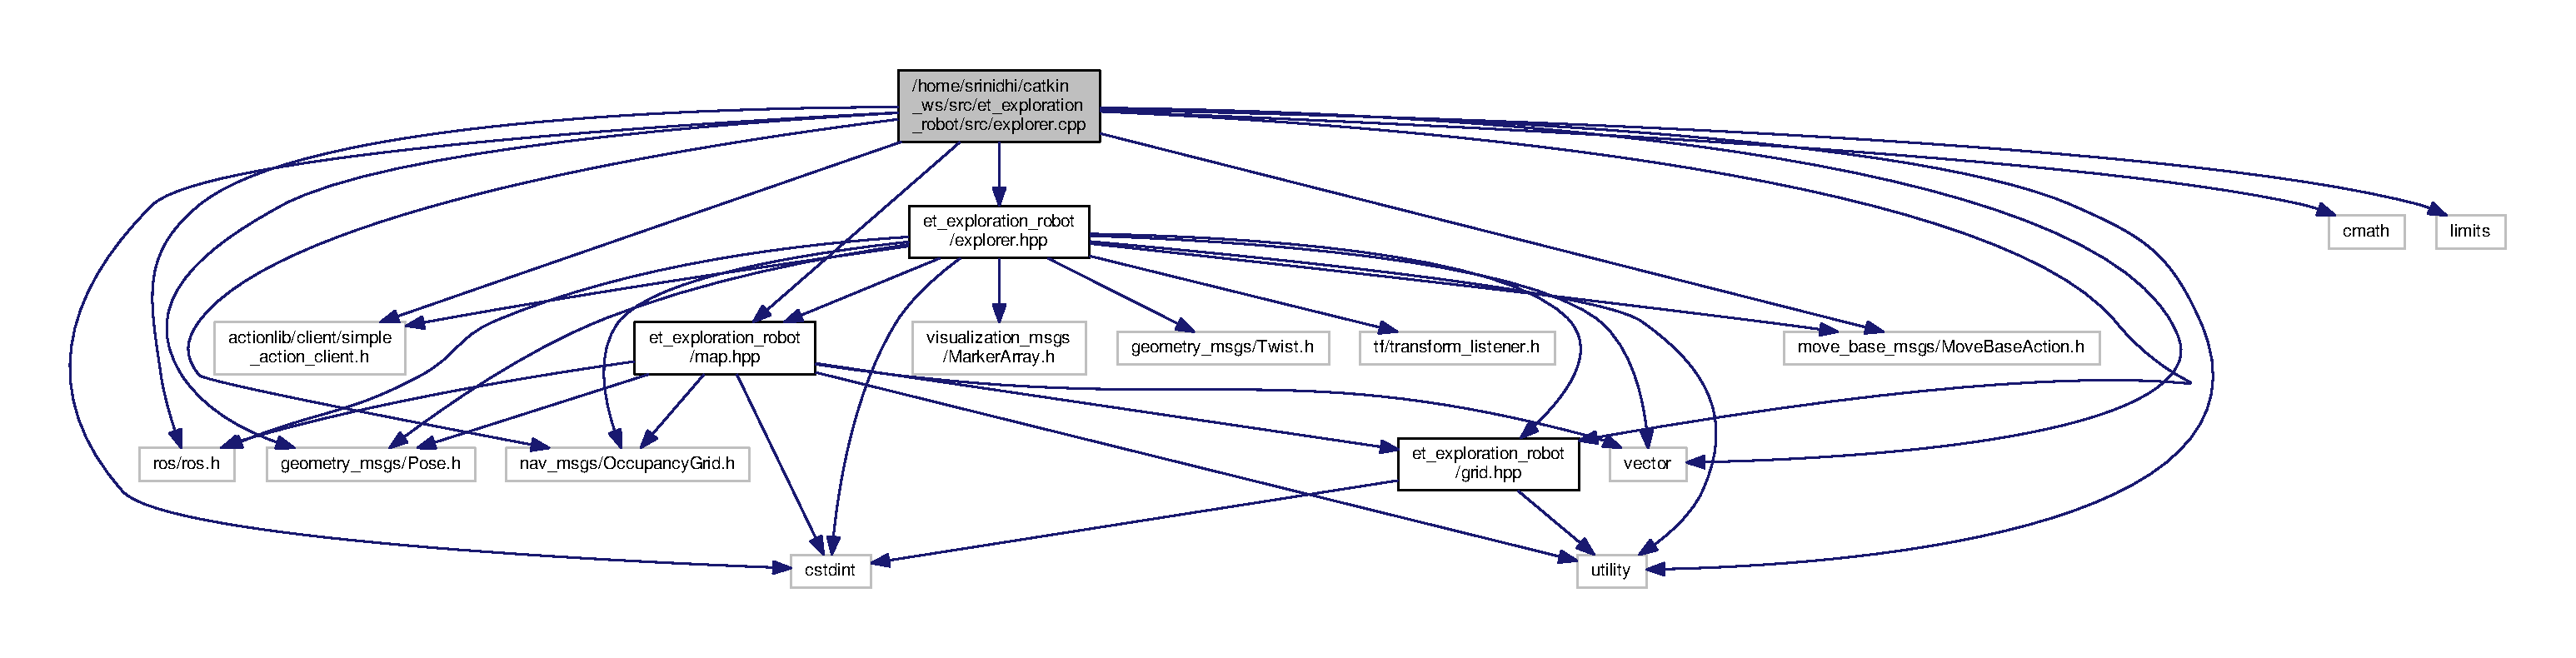
\includegraphics[width=350pt]{explorer_8cpp__incl}
\end{center}
\end{figure}


\subsection{Detailed Description}
\hyperlink{classExplorer}{Explorer} class method definitions. 

\begin{DoxyAuthor}{Author}
Srinidhi Sreenath (Srinidhi\+Sreenath) 
\end{DoxyAuthor}
\begin{DoxyDate}{Date}
12/15/2018 
\end{DoxyDate}
\begin{DoxyVersion}{Version}
1.\+0
\end{DoxyVersion}
\hypertarget{mapTest_8cpp_DESCRIPTION}{}\subsection{D\+E\+S\+C\+R\+I\+P\+T\+I\+ON}\label{mapTest_8cpp_DESCRIPTION}
Source file for class \hyperlink{classExplorer}{Explorer} which implements the exploration behavior for a turtlebot in an unknown environment. The turtlebot intially rotates in the environment and determines the frontiers i.\+e regions between explored and unexplored regions. It then navigates to closest reachable frontier and then restarts the rotation behavior to determine new frontiers. The behavior continues until the exploration is complete. 
\hypertarget{grid_8cpp}{}\section{/home/srinidhi/catkin\+\_\+ws/src/et\+\_\+exploration\+\_\+robot/src/grid.cpp File Reference}
\label{grid_8cpp}\index{/home/srinidhi/catkin\+\_\+ws/src/et\+\_\+exploration\+\_\+robot/src/grid.\+cpp@{/home/srinidhi/catkin\+\_\+ws/src/et\+\_\+exploration\+\_\+robot/src/grid.\+cpp}}


\hyperlink{classGrid}{Grid} class definitions.  


{\ttfamily \#include $<$cstdint$>$}\\*
{\ttfamily \#include $<$utility$>$}\\*
{\ttfamily \#include \char`\"{}et\+\_\+exploration\+\_\+robot/grid.\+hpp\char`\"{}}\\*
Include dependency graph for grid.\+cpp\+:
\nopagebreak
\begin{figure}[H]
\begin{center}
\leavevmode
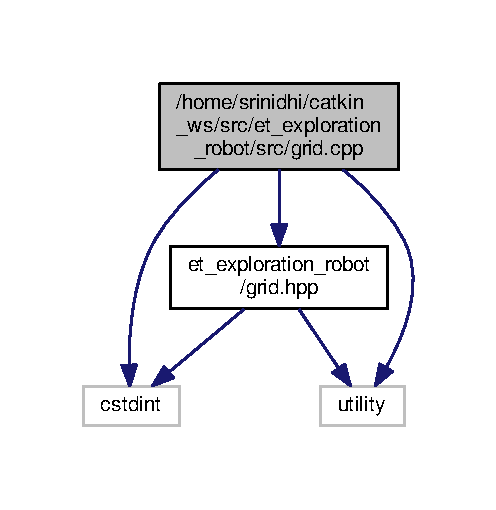
\includegraphics[width=238pt]{grid_8cpp__incl}
\end{center}
\end{figure}


\subsection{Detailed Description}
\hyperlink{classGrid}{Grid} class definitions. 

\begin{DoxyAuthor}{Author}
Srinidhi Sreenath (Srinidhi\+Sreenath) 
\end{DoxyAuthor}
\begin{DoxyDate}{Date}
12/15/2018 
\end{DoxyDate}
\begin{DoxyVersion}{Version}
1.\+0
\end{DoxyVersion}
\hypertarget{mapTest_8cpp_DESCRIPTION}{}\subsection{D\+E\+S\+C\+R\+I\+P\+T\+I\+ON}\label{mapTest_8cpp_DESCRIPTION}
Source file for class \hyperlink{classGrid}{Grid} which stores information of a single grid cell in the occupancy grid map. The class implements setter and getter function for the grid cell height, width coordinate. occupancy probability, frontier status and cluster number. 
\hypertarget{main_8cpp}{}\section{/home/srinidhi/catkin\+\_\+ws/src/et\+\_\+exploration\+\_\+robot/src/main.cpp File Reference}
\label{main_8cpp}\index{/home/srinidhi/catkin\+\_\+ws/src/et\+\_\+exploration\+\_\+robot/src/main.\+cpp@{/home/srinidhi/catkin\+\_\+ws/src/et\+\_\+exploration\+\_\+robot/src/main.\+cpp}}


Main source file.  


{\ttfamily \#include $<$ros/ros.\+h$>$}\\*
{\ttfamily \#include \char`\"{}et\+\_\+exploration\+\_\+robot/explorer.\+hpp\char`\"{}}\\*
{\ttfamily \#include \char`\"{}et\+\_\+exploration\+\_\+robot/grid.\+hpp\char`\"{}}\\*
{\ttfamily \#include \char`\"{}et\+\_\+exploration\+\_\+robot/map.\+hpp\char`\"{}}\\*
Include dependency graph for main.\+cpp\+:
\nopagebreak
\begin{figure}[H]
\begin{center}
\leavevmode
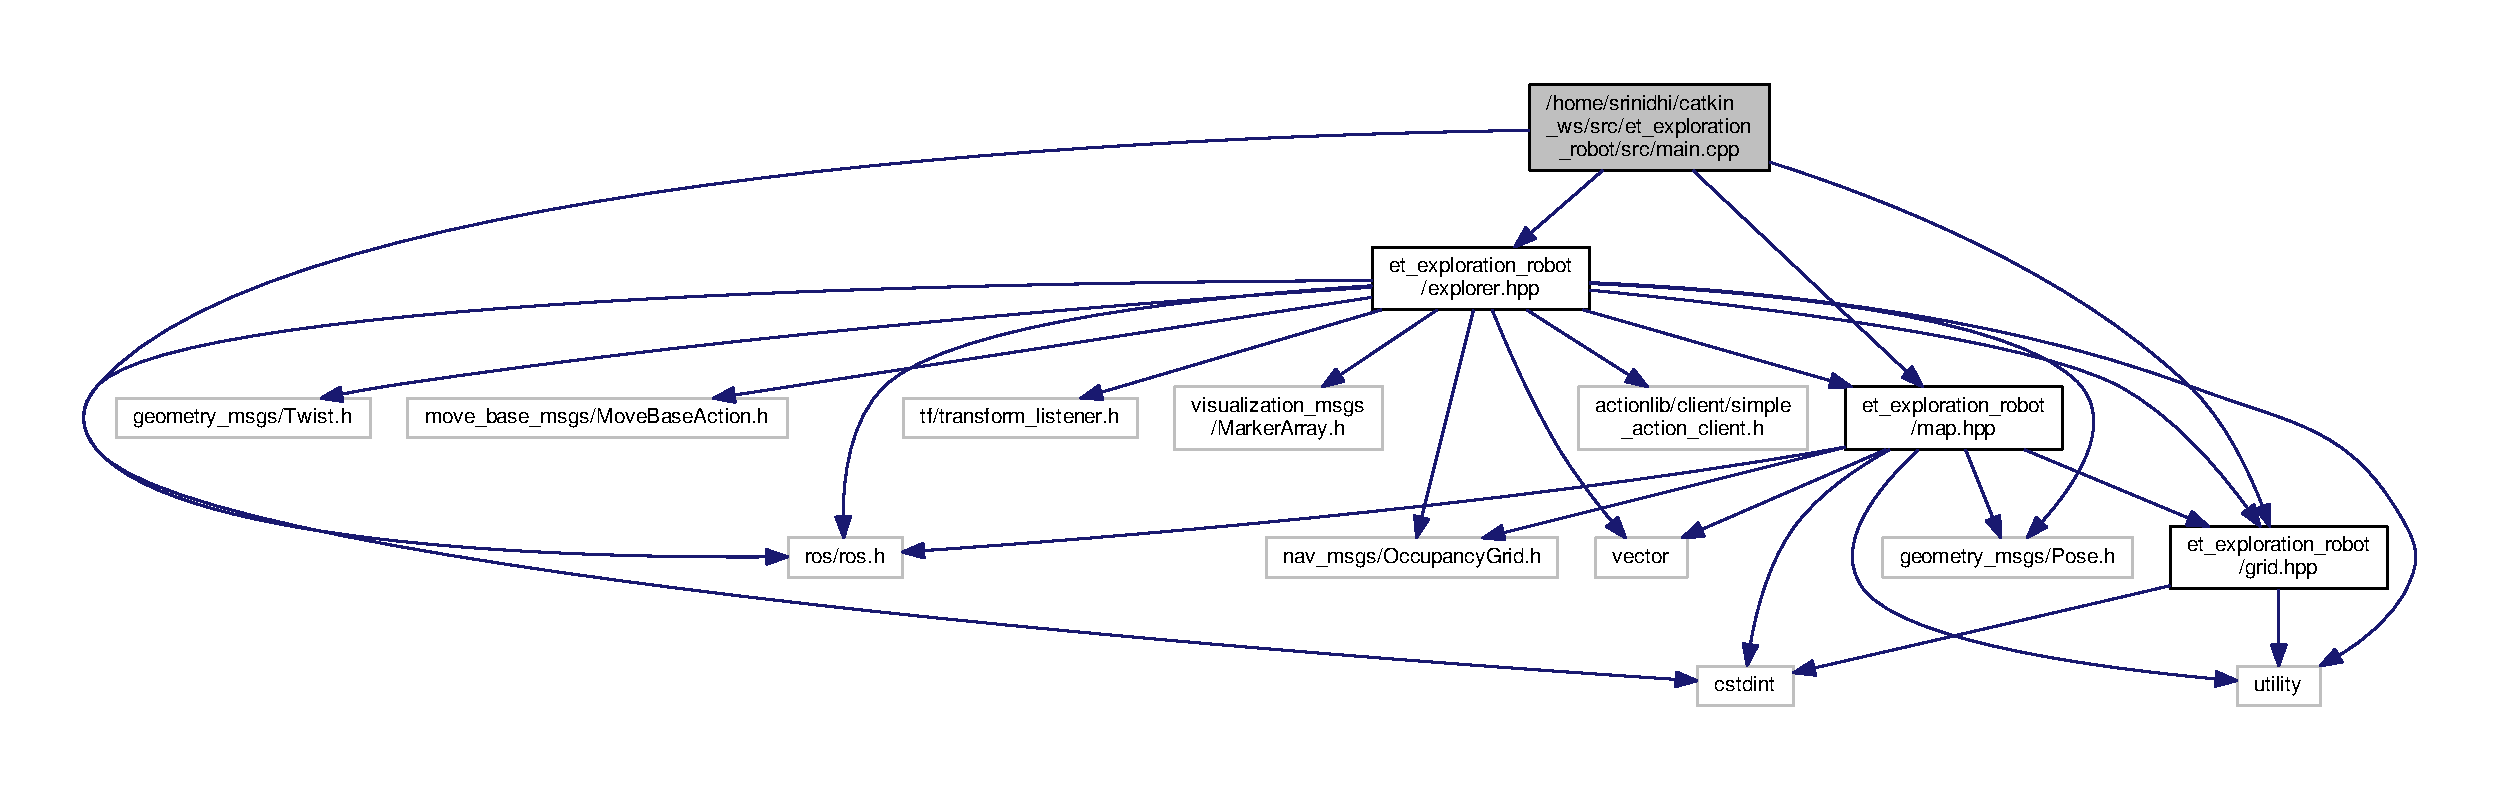
\includegraphics[width=350pt]{main_8cpp__incl}
\end{center}
\end{figure}
\subsection*{Functions}
\begin{DoxyCompactItemize}
\item 
int \hyperlink{main_8cpp_a3c04138a5bfe5d72780bb7e82a18e627}{main} (int argc, char $\ast$$\ast$argv)
\begin{DoxyCompactList}\small\item\em Main function to set up the R\+OS node and implement the exploration. \end{DoxyCompactList}\end{DoxyCompactItemize}


\subsection{Detailed Description}
Main source file. 

\begin{DoxyAuthor}{Author}
Srinidhi Sreenath (Srinidhi\+Sreenath) 
\end{DoxyAuthor}
\begin{DoxyDate}{Date}
12/15/2018 
\end{DoxyDate}
\begin{DoxyVersion}{Version}
1.\+0
\end{DoxyVersion}
\hypertarget{mapTest_8cpp_DESCRIPTION}{}\subsection{D\+E\+S\+C\+R\+I\+P\+T\+I\+ON}\label{mapTest_8cpp_DESCRIPTION}
Main source file to implement the exploration of an unknown environment using a turtlebot. 

\subsection{Function Documentation}
\index{main.\+cpp@{main.\+cpp}!main@{main}}
\index{main@{main}!main.\+cpp@{main.\+cpp}}
\subsubsection[{\texorpdfstring{main(int argc, char $\ast$$\ast$argv)}{main(int argc, char **argv)}}]{\setlength{\rightskip}{0pt plus 5cm}int main (
\begin{DoxyParamCaption}
\item[{int}]{argc, }
\item[{char $\ast$$\ast$}]{argv}
\end{DoxyParamCaption}
)}\hypertarget{main_8cpp_a3c04138a5bfe5d72780bb7e82a18e627}{}\label{main_8cpp_a3c04138a5bfe5d72780bb7e82a18e627}


Main function to set up the R\+OS node and implement the exploration. 


\begin{DoxyParams}{Parameters}
{\em argc} & -\/ argument count as integer \\
\hline
{\em argv} & -\/ argument vector as character array\\
\hline
\end{DoxyParams}
\begin{DoxyReturn}{Returns}
integer 0 indication successful execution 
\end{DoxyReturn}

\hypertarget{map_8cpp}{}\section{/home/srinidhi/catkin\+\_\+ws/src/et\+\_\+exploration\+\_\+robot/src/map.cpp File Reference}
\label{map_8cpp}\index{/home/srinidhi/catkin\+\_\+ws/src/et\+\_\+exploration\+\_\+robot/src/map.\+cpp@{/home/srinidhi/catkin\+\_\+ws/src/et\+\_\+exploration\+\_\+robot/src/map.\+cpp}}


\hyperlink{classMap}{Map} class definition.  


{\ttfamily \#include $<$geometry\+\_\+msgs/\+Pose.\+h$>$}\\*
{\ttfamily \#include $<$nav\+\_\+msgs/\+Occupancy\+Grid.\+h$>$}\\*
{\ttfamily \#include $<$ros/ros.\+h$>$}\\*
{\ttfamily \#include $<$cstdint$>$}\\*
{\ttfamily \#include $<$utility$>$}\\*
{\ttfamily \#include $<$vector$>$}\\*
{\ttfamily \#include \char`\"{}et\+\_\+exploration\+\_\+robot/grid.\+hpp\char`\"{}}\\*
{\ttfamily \#include \char`\"{}et\+\_\+exploration\+\_\+robot/map.\+hpp\char`\"{}}\\*
Include dependency graph for map.\+cpp\+:
\nopagebreak
\begin{figure}[H]
\begin{center}
\leavevmode
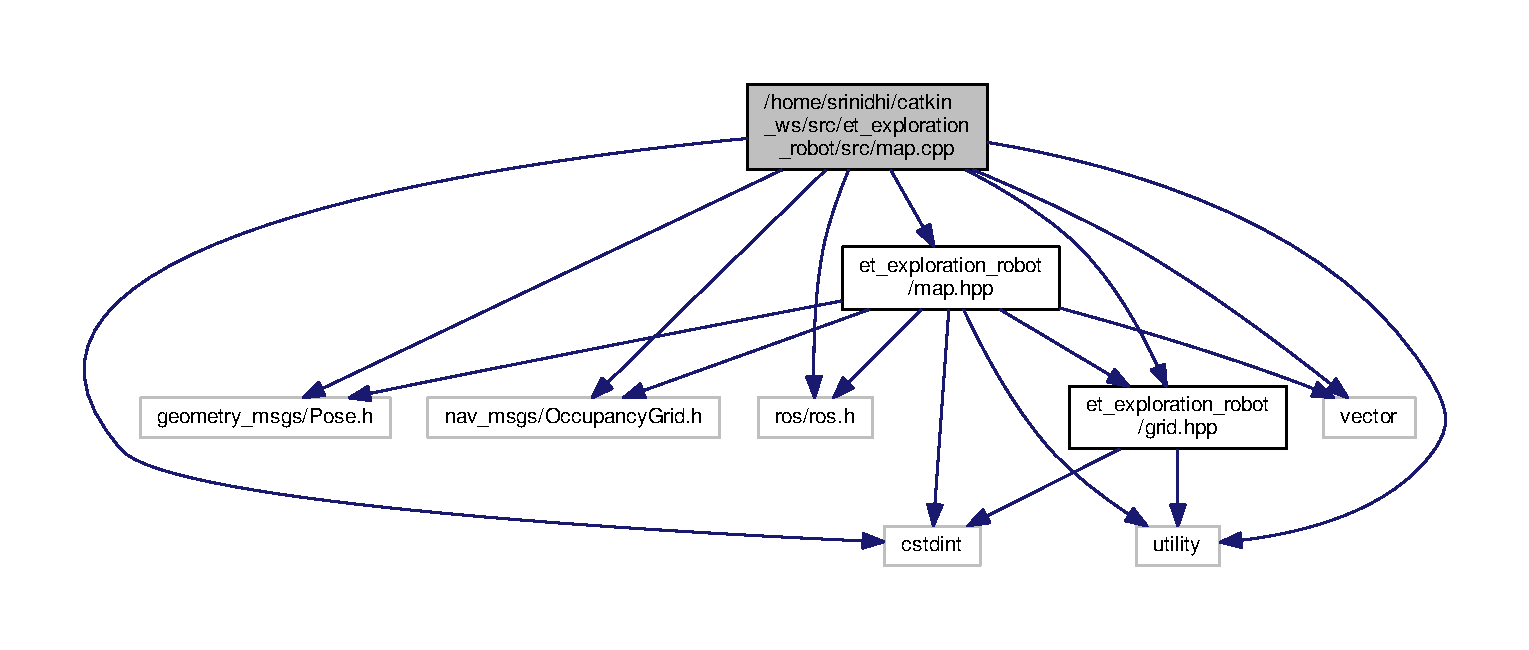
\includegraphics[width=350pt]{map_8cpp__incl}
\end{center}
\end{figure}


\subsection{Detailed Description}
\hyperlink{classMap}{Map} class definition. 

\begin{DoxyAuthor}{Author}
Srinidhi Sreenath (Srinidhi\+Sreenath) 
\end{DoxyAuthor}
\begin{DoxyDate}{Date}
12/15/2018 
\end{DoxyDate}
\begin{DoxyVersion}{Version}
1.\+0
\end{DoxyVersion}
\hypertarget{mapTest_8cpp_DESCRIPTION}{}\subsection{D\+E\+S\+C\+R\+I\+P\+T\+I\+ON}\label{mapTest_8cpp_DESCRIPTION}
Source file for class \hyperlink{classMap}{Map} which stores the occupancy grid map information. The class also implements methods to determine the frontier grid cells and cluster them. It also has helper function to convert from occupancy grid coordinates to cartesian coordinates. 
\hypertarget{explorerTest_8cpp}{}\section{/home/srinidhi/catkin\+\_\+ws/src/et\+\_\+exploration\+\_\+robot/test/explorer\+Test.cpp File Reference}
\label{explorerTest_8cpp}\index{/home/srinidhi/catkin\+\_\+ws/src/et\+\_\+exploration\+\_\+robot/test/explorer\+Test.\+cpp@{/home/srinidhi/catkin\+\_\+ws/src/et\+\_\+exploration\+\_\+robot/test/explorer\+Test.\+cpp}}


Rostests for class \hyperlink{classExplorer}{Explorer}.  


{\ttfamily \#include $<$gtest/gtest.\+h$>$}\\*
{\ttfamily \#include $<$ros/ros.\+h$>$}\\*
{\ttfamily \#include $<$cstdint$>$}\\*
{\ttfamily \#include $<$utility$>$}\\*
{\ttfamily \#include $<$vector$>$}\\*
{\ttfamily \#include \char`\"{}et\+\_\+exploration\+\_\+robot/explorer.\+hpp\char`\"{}}\\*
{\ttfamily \#include \char`\"{}et\+\_\+exploration\+\_\+robot/grid.\+hpp\char`\"{}}\\*
{\ttfamily \#include \char`\"{}et\+\_\+exploration\+\_\+robot/map.\+hpp\char`\"{}}\\*
Include dependency graph for explorer\+Test.\+cpp\+:
\nopagebreak
\begin{figure}[H]
\begin{center}
\leavevmode
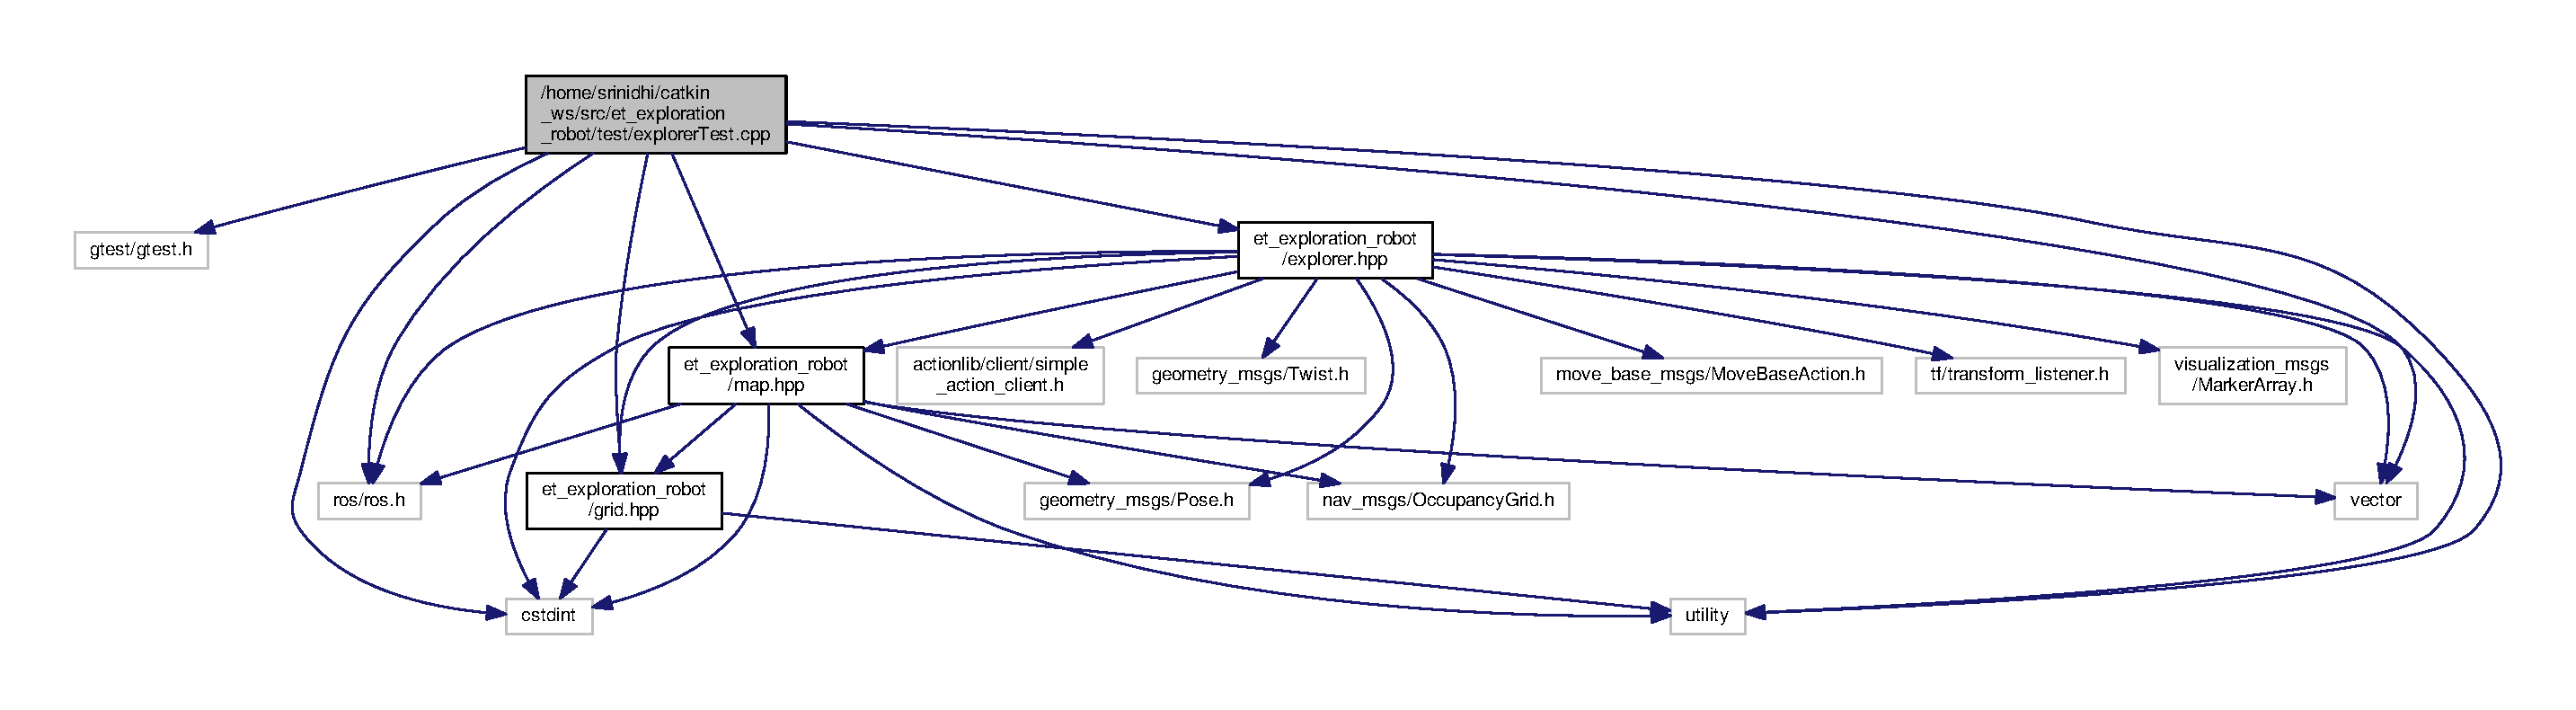
\includegraphics[width=350pt]{explorerTest_8cpp__incl}
\end{center}
\end{figure}
\subsection*{Classes}
\begin{DoxyCompactItemize}
\item 
class \hyperlink{classTestPub}{Test\+Pub}
\begin{DoxyCompactList}\small\item\em Class \hyperlink{classTestPub}{Test\+Pub}. \end{DoxyCompactList}\item 
class \hyperlink{classExplorerTest}{Explorer\+Test}
\begin{DoxyCompactList}\small\item\em Class \hyperlink{classExplorerTest}{Explorer\+Test}. \end{DoxyCompactList}\end{DoxyCompactItemize}
\subsection*{Functions}
\begin{DoxyCompactItemize}
\item 
\hyperlink{explorerTest_8cpp_a43780f388580a5ccad8263ef48983d00}{T\+E\+S\+T\+\_\+F} (\hyperlink{classExplorerTest}{Explorer\+Test}, test\+Velocity\+Publisher)
\begin{DoxyCompactList}\small\item\em Test case to check if the velocity publisher is set up with R\+OS Master when the explorer class is initialized. \end{DoxyCompactList}\item 
\hyperlink{explorerTest_8cpp_a5dc444be2ffdb362062b16e701d8b24b}{T\+E\+S\+T\+\_\+F} (\hyperlink{classExplorerTest}{Explorer\+Test}, test\+Marker\+Publisher)
\begin{DoxyCompactList}\small\item\em Test case to check if the markerarray publisher is set up with R\+OS Master when the explorer class is initialized. \end{DoxyCompactList}\item 
\hyperlink{explorerTest_8cpp_ac0f4c28896dde82dd86c3e311c172adc}{T\+E\+S\+T\+\_\+F} (\hyperlink{classExplorerTest}{Explorer\+Test}, test\+Map\+Subscriber)
\begin{DoxyCompactList}\small\item\em Test case to check if the map subcriber is set up when the explorer class is initialized. \end{DoxyCompactList}\end{DoxyCompactItemize}


\subsection{Detailed Description}
Rostests for class \hyperlink{classExplorer}{Explorer}. 

\begin{DoxyAuthor}{Author}
Srinidhi Sreenath (Srinidhi\+Sreenath) 
\end{DoxyAuthor}
\begin{DoxyDate}{Date}
12/15/2018 
\end{DoxyDate}
\begin{DoxyVersion}{Version}
1.\+0
\end{DoxyVersion}
\hypertarget{mapTest_8cpp_DESCRIPTION}{}\subsection{D\+E\+S\+C\+R\+I\+P\+T\+I\+ON}\label{mapTest_8cpp_DESCRIPTION}
Test cases to test subscribers and publishers in class \hyperlink{classExplorer}{Explorer} 

\subsection{Function Documentation}
\index{explorer\+Test.\+cpp@{explorer\+Test.\+cpp}!T\+E\+S\+T\+\_\+F@{T\+E\+S\+T\+\_\+F}}
\index{T\+E\+S\+T\+\_\+F@{T\+E\+S\+T\+\_\+F}!explorer\+Test.\+cpp@{explorer\+Test.\+cpp}}
\subsubsection[{\texorpdfstring{T\+E\+S\+T\+\_\+\+F(\+Explorer\+Test, test\+Velocity\+Publisher)}{TEST_F(ExplorerTest, testVelocityPublisher)}}]{\setlength{\rightskip}{0pt plus 5cm}T\+E\+S\+T\+\_\+F (
\begin{DoxyParamCaption}
\item[{{\bf Explorer\+Test}}]{, }
\item[{test\+Velocity\+Publisher}]{}
\end{DoxyParamCaption}
)}\hypertarget{explorerTest_8cpp_a43780f388580a5ccad8263ef48983d00}{}\label{explorerTest_8cpp_a43780f388580a5ccad8263ef48983d00}


Test case to check if the velocity publisher is set up with R\+OS Master when the explorer class is initialized. 


\begin{DoxyParams}{Parameters}
{\em \hyperlink{classExplorerTest}{Explorer\+Test}} & -\/ gtest framwork for test fixtures \\
\hline
{\em test\+Velocity\+Publisher} & -\/ test name\\
\hline
\end{DoxyParams}
\begin{DoxyReturn}{Returns}
void 
\end{DoxyReturn}
\index{explorer\+Test.\+cpp@{explorer\+Test.\+cpp}!T\+E\+S\+T\+\_\+F@{T\+E\+S\+T\+\_\+F}}
\index{T\+E\+S\+T\+\_\+F@{T\+E\+S\+T\+\_\+F}!explorer\+Test.\+cpp@{explorer\+Test.\+cpp}}
\subsubsection[{\texorpdfstring{T\+E\+S\+T\+\_\+\+F(\+Explorer\+Test, test\+Marker\+Publisher)}{TEST_F(ExplorerTest, testMarkerPublisher)}}]{\setlength{\rightskip}{0pt plus 5cm}T\+E\+S\+T\+\_\+F (
\begin{DoxyParamCaption}
\item[{{\bf Explorer\+Test}}]{, }
\item[{test\+Marker\+Publisher}]{}
\end{DoxyParamCaption}
)}\hypertarget{explorerTest_8cpp_a5dc444be2ffdb362062b16e701d8b24b}{}\label{explorerTest_8cpp_a5dc444be2ffdb362062b16e701d8b24b}


Test case to check if the markerarray publisher is set up with R\+OS Master when the explorer class is initialized. 


\begin{DoxyParams}{Parameters}
{\em \hyperlink{classExplorerTest}{Explorer\+Test}} & -\/ gtest framwork for test fixtures \\
\hline
{\em test\+Marker\+Publisher} & -\/ test name\\
\hline
\end{DoxyParams}
\begin{DoxyReturn}{Returns}
void 
\end{DoxyReturn}
\index{explorer\+Test.\+cpp@{explorer\+Test.\+cpp}!T\+E\+S\+T\+\_\+F@{T\+E\+S\+T\+\_\+F}}
\index{T\+E\+S\+T\+\_\+F@{T\+E\+S\+T\+\_\+F}!explorer\+Test.\+cpp@{explorer\+Test.\+cpp}}
\subsubsection[{\texorpdfstring{T\+E\+S\+T\+\_\+\+F(\+Explorer\+Test, test\+Map\+Subscriber)}{TEST_F(ExplorerTest, testMapSubscriber)}}]{\setlength{\rightskip}{0pt plus 5cm}T\+E\+S\+T\+\_\+F (
\begin{DoxyParamCaption}
\item[{{\bf Explorer\+Test}}]{, }
\item[{test\+Map\+Subscriber}]{}
\end{DoxyParamCaption}
)}\hypertarget{explorerTest_8cpp_ac0f4c28896dde82dd86c3e311c172adc}{}\label{explorerTest_8cpp_ac0f4c28896dde82dd86c3e311c172adc}


Test case to check if the map subcriber is set up when the explorer class is initialized. 


\begin{DoxyParams}{Parameters}
{\em \hyperlink{classExplorerTest}{Explorer\+Test}} & -\/ gtest framwork for test fixtures \\
\hline
{\em test\+Map\+Subscriber} & -\/ test name\\
\hline
\end{DoxyParams}
\begin{DoxyReturn}{Returns}
void 
\end{DoxyReturn}

\hypertarget{gridTest_8cpp}{}\section{/home/srinidhi/catkin\+\_\+ws/src/et\+\_\+exploration\+\_\+robot/test/grid\+Test.cpp File Reference}
\label{gridTest_8cpp}\index{/home/srinidhi/catkin\+\_\+ws/src/et\+\_\+exploration\+\_\+robot/test/grid\+Test.\+cpp@{/home/srinidhi/catkin\+\_\+ws/src/et\+\_\+exploration\+\_\+robot/test/grid\+Test.\+cpp}}


Unit tests for class \hyperlink{classGrid}{Grid}.  


{\ttfamily \#include $<$gtest/gtest.\+h$>$}\\*
{\ttfamily \#include $<$ros/ros.\+h$>$}\\*
{\ttfamily \#include $<$cstdint$>$}\\*
{\ttfamily \#include $<$utility$>$}\\*
{\ttfamily \#include \char`\"{}et\+\_\+exploration\+\_\+robot/grid.\+hpp\char`\"{}}\\*
Include dependency graph for grid\+Test.\+cpp\+:
\nopagebreak
\begin{figure}[H]
\begin{center}
\leavevmode
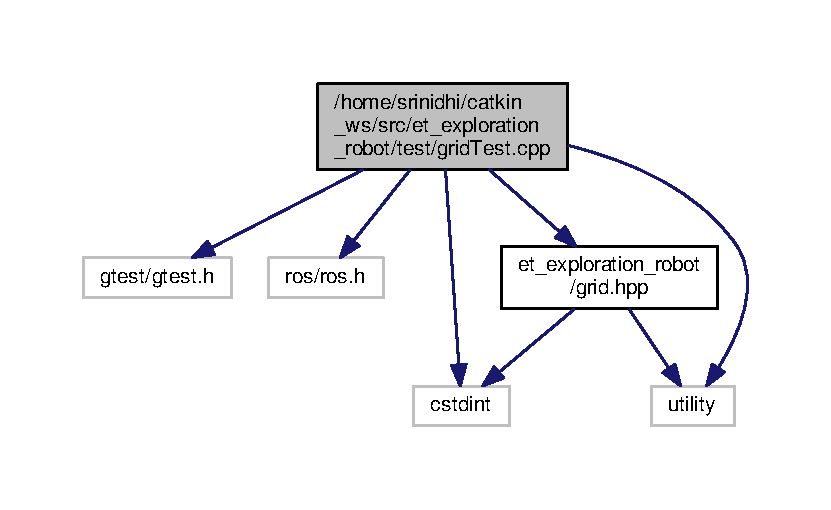
\includegraphics[width=350pt]{gridTest_8cpp__incl}
\end{center}
\end{figure}
\subsection*{Classes}
\begin{DoxyCompactItemize}
\item 
class \hyperlink{classGridTest}{Grid\+Test}
\begin{DoxyCompactList}\small\item\em Class \hyperlink{classGridTest}{Grid\+Test}. \end{DoxyCompactList}\end{DoxyCompactItemize}
\subsection*{Functions}
\begin{DoxyCompactItemize}
\item 
\hyperlink{gridTest_8cpp_a7e5f531ceac3ae0d08cac5cda0b9241f}{T\+E\+S\+T\+\_\+F} (\hyperlink{classGridTest}{Grid\+Test}, test\+Setting\+Grid\+State)
\begin{DoxyCompactList}\small\item\em Test case to check setting and getting the grid cell state. \end{DoxyCompactList}\item 
\hyperlink{gridTest_8cpp_a71100157e4b6d934ed9e53a6669600e9}{T\+E\+S\+T\+\_\+F} (\hyperlink{classGridTest}{Grid\+Test}, test\+Updating\+Grid\+Probability)
\begin{DoxyCompactList}\small\item\em Test case to check updating and obtaining the probability of the grid cell. \end{DoxyCompactList}\item 
\hyperlink{gridTest_8cpp_a10b5c909712149b8e02e9a2c8cb8ff46}{T\+E\+S\+T\+\_\+F} (\hyperlink{classGridTest}{Grid\+Test}, test\+Setting\+Grid\+Frontier\+Status)
\begin{DoxyCompactList}\small\item\em Test case to check setting and obtaining the frontier status of the grid cell. \end{DoxyCompactList}\item 
\hyperlink{gridTest_8cpp_aa6d541d707a3ad8f9591302cc46c79af}{T\+E\+S\+T\+\_\+F} (\hyperlink{classGridTest}{Grid\+Test}, test\+Setting\+Grid\+Cluster)
\begin{DoxyCompactList}\small\item\em Test case to check setting and obtaining the cluster number of the grid cell. \end{DoxyCompactList}\end{DoxyCompactItemize}


\subsection{Detailed Description}
Unit tests for class \hyperlink{classGrid}{Grid}. 

\begin{DoxyAuthor}{Author}
Srinidhi Sreenath (Srinidhi\+Sreenath) 
\end{DoxyAuthor}
\begin{DoxyDate}{Date}
12/15/2018 
\end{DoxyDate}
\begin{DoxyVersion}{Version}
1.\+0
\end{DoxyVersion}
\hypertarget{mapTest_8cpp_DESCRIPTION}{}\subsection{D\+E\+S\+C\+R\+I\+P\+T\+I\+ON}\label{mapTest_8cpp_DESCRIPTION}
Test cases to test member functions of class \hyperlink{classGrid}{Grid}. 

\subsection{Function Documentation}
\index{grid\+Test.\+cpp@{grid\+Test.\+cpp}!T\+E\+S\+T\+\_\+F@{T\+E\+S\+T\+\_\+F}}
\index{T\+E\+S\+T\+\_\+F@{T\+E\+S\+T\+\_\+F}!grid\+Test.\+cpp@{grid\+Test.\+cpp}}
\subsubsection[{\texorpdfstring{T\+E\+S\+T\+\_\+\+F(\+Grid\+Test, test\+Setting\+Grid\+State)}{TEST_F(GridTest, testSettingGridState)}}]{\setlength{\rightskip}{0pt plus 5cm}T\+E\+S\+T\+\_\+F (
\begin{DoxyParamCaption}
\item[{{\bf Grid\+Test}}]{, }
\item[{test\+Setting\+Grid\+State}]{}
\end{DoxyParamCaption}
)}\hypertarget{gridTest_8cpp_a7e5f531ceac3ae0d08cac5cda0b9241f}{}\label{gridTest_8cpp_a7e5f531ceac3ae0d08cac5cda0b9241f}


Test case to check setting and getting the grid cell state. 


\begin{DoxyParams}{Parameters}
{\em \hyperlink{classGridTest}{Grid\+Test}} & -\/ gtest framwork for test fixtures \\
\hline
{\em test\+Setting\+Grid\+State} & -\/ test name\\
\hline
\end{DoxyParams}
\begin{DoxyReturn}{Returns}
void 
\end{DoxyReturn}
\index{grid\+Test.\+cpp@{grid\+Test.\+cpp}!T\+E\+S\+T\+\_\+F@{T\+E\+S\+T\+\_\+F}}
\index{T\+E\+S\+T\+\_\+F@{T\+E\+S\+T\+\_\+F}!grid\+Test.\+cpp@{grid\+Test.\+cpp}}
\subsubsection[{\texorpdfstring{T\+E\+S\+T\+\_\+\+F(\+Grid\+Test, test\+Updating\+Grid\+Probability)}{TEST_F(GridTest, testUpdatingGridProbability)}}]{\setlength{\rightskip}{0pt plus 5cm}T\+E\+S\+T\+\_\+F (
\begin{DoxyParamCaption}
\item[{{\bf Grid\+Test}}]{, }
\item[{test\+Updating\+Grid\+Probability}]{}
\end{DoxyParamCaption}
)}\hypertarget{gridTest_8cpp_a71100157e4b6d934ed9e53a6669600e9}{}\label{gridTest_8cpp_a71100157e4b6d934ed9e53a6669600e9}


Test case to check updating and obtaining the probability of the grid cell. 


\begin{DoxyParams}{Parameters}
{\em \hyperlink{classGridTest}{Grid\+Test}} & -\/ gtest framwork for test fixtures \\
\hline
{\em test\+Updating\+Grid\+Probability} & -\/ test name\\
\hline
\end{DoxyParams}
\begin{DoxyReturn}{Returns}
void 
\end{DoxyReturn}
\index{grid\+Test.\+cpp@{grid\+Test.\+cpp}!T\+E\+S\+T\+\_\+F@{T\+E\+S\+T\+\_\+F}}
\index{T\+E\+S\+T\+\_\+F@{T\+E\+S\+T\+\_\+F}!grid\+Test.\+cpp@{grid\+Test.\+cpp}}
\subsubsection[{\texorpdfstring{T\+E\+S\+T\+\_\+\+F(\+Grid\+Test, test\+Setting\+Grid\+Frontier\+Status)}{TEST_F(GridTest, testSettingGridFrontierStatus)}}]{\setlength{\rightskip}{0pt plus 5cm}T\+E\+S\+T\+\_\+F (
\begin{DoxyParamCaption}
\item[{{\bf Grid\+Test}}]{, }
\item[{test\+Setting\+Grid\+Frontier\+Status}]{}
\end{DoxyParamCaption}
)}\hypertarget{gridTest_8cpp_a10b5c909712149b8e02e9a2c8cb8ff46}{}\label{gridTest_8cpp_a10b5c909712149b8e02e9a2c8cb8ff46}


Test case to check setting and obtaining the frontier status of the grid cell. 


\begin{DoxyParams}{Parameters}
{\em \hyperlink{classGridTest}{Grid\+Test}} & -\/ gtest framwork for test fixtures \\
\hline
{\em test\+Setting\+Grid\+Frontier\+Status} & -\/ test name\\
\hline
\end{DoxyParams}
\begin{DoxyReturn}{Returns}
void 
\end{DoxyReturn}
\index{grid\+Test.\+cpp@{grid\+Test.\+cpp}!T\+E\+S\+T\+\_\+F@{T\+E\+S\+T\+\_\+F}}
\index{T\+E\+S\+T\+\_\+F@{T\+E\+S\+T\+\_\+F}!grid\+Test.\+cpp@{grid\+Test.\+cpp}}
\subsubsection[{\texorpdfstring{T\+E\+S\+T\+\_\+\+F(\+Grid\+Test, test\+Setting\+Grid\+Cluster)}{TEST_F(GridTest, testSettingGridCluster)}}]{\setlength{\rightskip}{0pt plus 5cm}T\+E\+S\+T\+\_\+F (
\begin{DoxyParamCaption}
\item[{{\bf Grid\+Test}}]{, }
\item[{test\+Setting\+Grid\+Cluster}]{}
\end{DoxyParamCaption}
)}\hypertarget{gridTest_8cpp_aa6d541d707a3ad8f9591302cc46c79af}{}\label{gridTest_8cpp_aa6d541d707a3ad8f9591302cc46c79af}


Test case to check setting and obtaining the cluster number of the grid cell. 


\begin{DoxyParams}{Parameters}
{\em \hyperlink{classGridTest}{Grid\+Test}} & -\/ gtest framwork for test fixtures \\
\hline
{\em test\+Setting\+Grid\+Cluster} & -\/ test name\\
\hline
\end{DoxyParams}
\begin{DoxyReturn}{Returns}
void 
\end{DoxyReturn}

\hypertarget{mainTest_8cpp}{}\section{/home/srinidhi/catkin\+\_\+ws/src/et\+\_\+exploration\+\_\+robot/test/main\+Test.cpp File Reference}
\label{mainTest_8cpp}\index{/home/srinidhi/catkin\+\_\+ws/src/et\+\_\+exploration\+\_\+robot/test/main\+Test.\+cpp@{/home/srinidhi/catkin\+\_\+ws/src/et\+\_\+exploration\+\_\+robot/test/main\+Test.\+cpp}}


Main file to run all unit tests and rostests.  


{\ttfamily \#include $<$gtest/gtest.\+h$>$}\\*
{\ttfamily \#include $<$ros/ros.\+h$>$}\\*
Include dependency graph for main\+Test.\+cpp\+:
\nopagebreak
\begin{figure}[H]
\begin{center}
\leavevmode
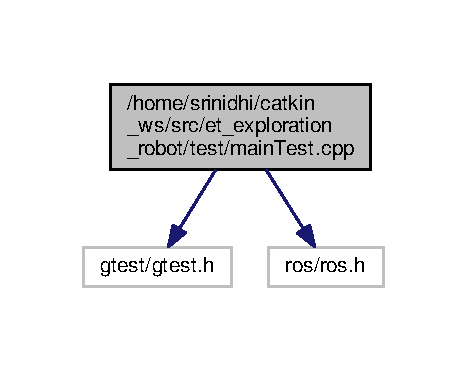
\includegraphics[width=224pt]{mainTest_8cpp__incl}
\end{center}
\end{figure}
\subsection*{Functions}
\begin{DoxyCompactItemize}
\item 
int \hyperlink{mainTest_8cpp_a3c04138a5bfe5d72780bb7e82a18e627}{main} (int argc, char $\ast$$\ast$argv)
\begin{DoxyCompactList}\small\item\em Run all google unit tests. \end{DoxyCompactList}\end{DoxyCompactItemize}


\subsection{Detailed Description}
Main file to run all unit tests and rostests. 

\begin{DoxyAuthor}{Author}
Srinidhi Sreenath (Srinidhi\+Sreenath) 
\end{DoxyAuthor}
\begin{DoxyDate}{Date}
12/15/2018 
\end{DoxyDate}
\begin{DoxyVersion}{Version}
1.\+0 
\end{DoxyVersion}


\subsection{Function Documentation}
\index{main\+Test.\+cpp@{main\+Test.\+cpp}!main@{main}}
\index{main@{main}!main\+Test.\+cpp@{main\+Test.\+cpp}}
\subsubsection[{\texorpdfstring{main(int argc, char $\ast$$\ast$argv)}{main(int argc, char **argv)}}]{\setlength{\rightskip}{0pt plus 5cm}int main (
\begin{DoxyParamCaption}
\item[{int}]{argc, }
\item[{char $\ast$$\ast$}]{argv}
\end{DoxyParamCaption}
)}\hypertarget{mainTest_8cpp_a3c04138a5bfe5d72780bb7e82a18e627}{}\label{mainTest_8cpp_a3c04138a5bfe5d72780bb7e82a18e627}


Run all google unit tests. 


\begin{DoxyParams}{Parameters}
{\em none} & \\
\hline
\end{DoxyParams}
\begin{DoxyReturn}{Returns}
0 on successful exit 
\end{DoxyReturn}

\hypertarget{mapTest_8cpp}{}\section{/home/srinidhi/catkin\+\_\+ws/src/et\+\_\+exploration\+\_\+robot/test/map\+Test.cpp File Reference}
\label{mapTest_8cpp}\index{/home/srinidhi/catkin\+\_\+ws/src/et\+\_\+exploration\+\_\+robot/test/map\+Test.\+cpp@{/home/srinidhi/catkin\+\_\+ws/src/et\+\_\+exploration\+\_\+robot/test/map\+Test.\+cpp}}


Unit tests for class \hyperlink{classMap}{Map}.  


{\ttfamily \#include $<$gtest/gtest.\+h$>$}\\*
{\ttfamily \#include $<$nav\+\_\+msgs/\+Map\+Meta\+Data.\+h$>$}\\*
{\ttfamily \#include $<$nav\+\_\+msgs/\+Occupancy\+Grid.\+h$>$}\\*
{\ttfamily \#include $<$ros/ros.\+h$>$}\\*
{\ttfamily \#include $<$cstdint$>$}\\*
{\ttfamily \#include $<$utility$>$}\\*
{\ttfamily \#include $<$vector$>$}\\*
{\ttfamily \#include \char`\"{}et\+\_\+exploration\+\_\+robot/grid.\+hpp\char`\"{}}\\*
{\ttfamily \#include \char`\"{}et\+\_\+exploration\+\_\+robot/map.\+hpp\char`\"{}}\\*
Include dependency graph for map\+Test.\+cpp\+:
\nopagebreak
\begin{figure}[H]
\begin{center}
\leavevmode
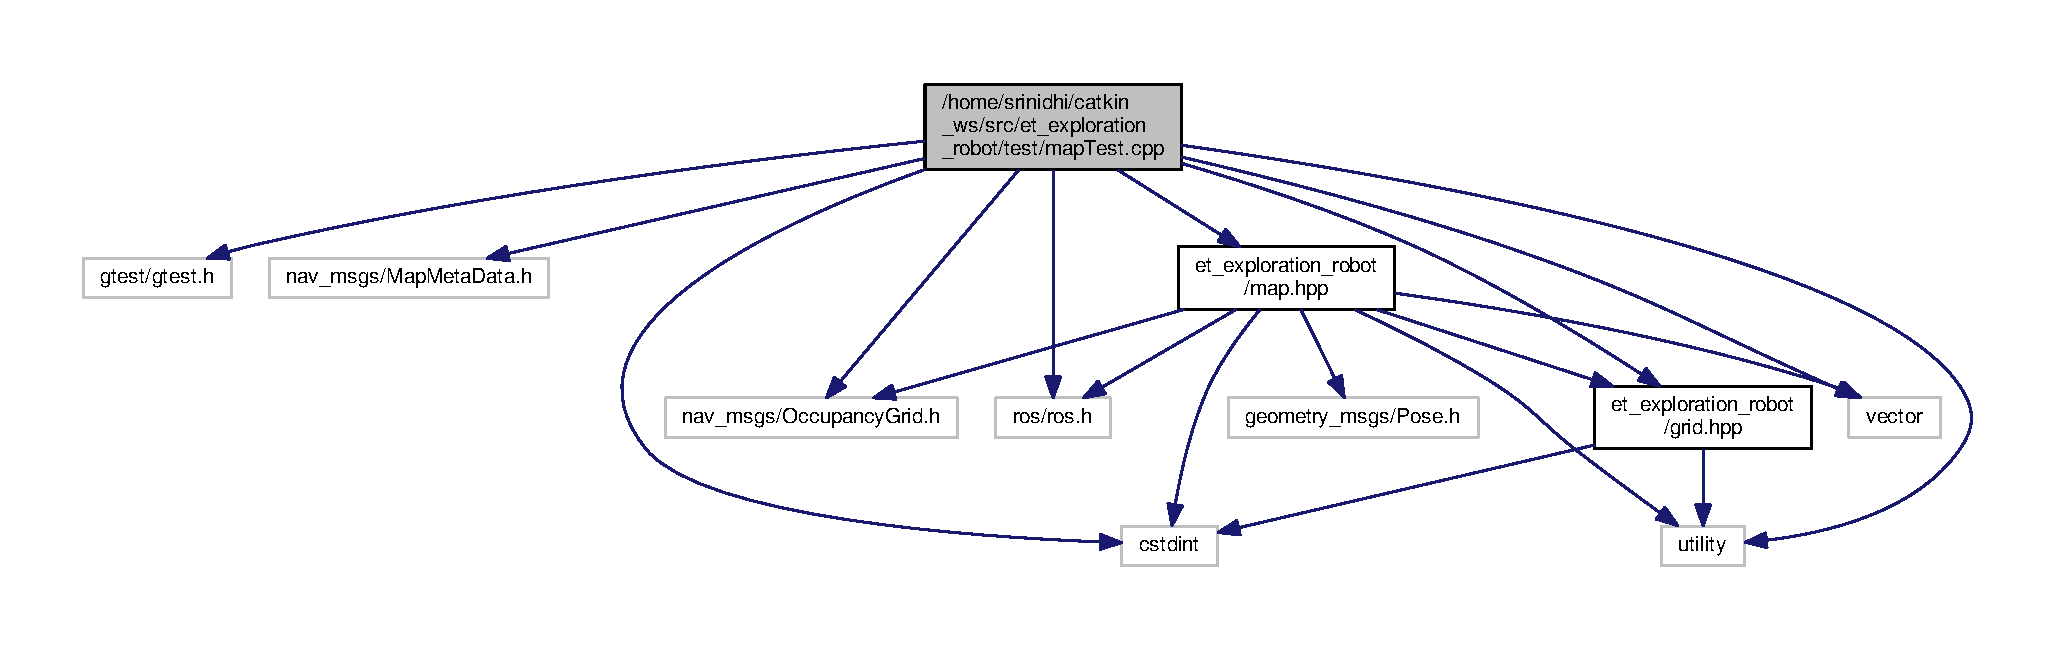
\includegraphics[width=350pt]{mapTest_8cpp__incl}
\end{center}
\end{figure}
\subsection*{Classes}
\begin{DoxyCompactItemize}
\item 
class \hyperlink{classMapTest}{Map\+Test}
\begin{DoxyCompactList}\small\item\em Class \hyperlink{classMapTest}{Map\+Test}. \end{DoxyCompactList}\end{DoxyCompactItemize}
\subsection*{Functions}
\begin{DoxyCompactItemize}
\item 
\hyperlink{mapTest_8cpp_a5f3421c12d094aef1f16c1f091be0fb9}{T\+E\+S\+T\+\_\+F} (\hyperlink{classMapTest}{Map\+Test}, test\+Initialization\+And\+Updation\+Of\+Map)
\begin{DoxyCompactList}\small\item\em Test case to check initialization and updation of occupancy map dimensions and parameters. \end{DoxyCompactList}\item 
\hyperlink{mapTest_8cpp_af3b36efb03d0f8eac404640b25f7cf12}{T\+E\+S\+T\+\_\+F} (\hyperlink{classMapTest}{Map\+Test}, test\+Frontier\+Clusters)
\begin{DoxyCompactList}\small\item\em Test case to check clustering of frontier cells. \end{DoxyCompactList}\item 
\hyperlink{mapTest_8cpp_a2480a94eed87bfa2fdc65516aaafed79}{T\+E\+S\+T\+\_\+F} (\hyperlink{classMapTest}{Map\+Test}, test\+Frontier\+Clusters\+Centroid)
\begin{DoxyCompactList}\small\item\em Test case to validate centroid of each frontier cluster. \end{DoxyCompactList}\item 
\hyperlink{mapTest_8cpp_a706cb0c20b34cdcb38f74c06d64b6d34}{T\+E\+S\+T\+\_\+F} (\hyperlink{classMapTest}{Map\+Test}, test\+Grid\+To\+Cartesian\+Conversion)
\begin{DoxyCompactList}\small\item\em Test case to check conversion from grid coordinates to cartesian coordinates. \end{DoxyCompactList}\end{DoxyCompactItemize}


\subsection{Detailed Description}
Unit tests for class \hyperlink{classMap}{Map}. 

\begin{DoxyAuthor}{Author}
Srinidhi Sreenath (Srinidhi\+Sreenath) 
\end{DoxyAuthor}
\begin{DoxyDate}{Date}
12/15/2018 
\end{DoxyDate}
\begin{DoxyVersion}{Version}
1.\+0
\end{DoxyVersion}
\hypertarget{mapTest_8cpp_DESCRIPTION}{}\subsection{D\+E\+S\+C\+R\+I\+P\+T\+I\+ON}\label{mapTest_8cpp_DESCRIPTION}
Test cases to test member functions of class \hyperlink{classMap}{Map}. 

\subsection{Function Documentation}
\index{map\+Test.\+cpp@{map\+Test.\+cpp}!T\+E\+S\+T\+\_\+F@{T\+E\+S\+T\+\_\+F}}
\index{T\+E\+S\+T\+\_\+F@{T\+E\+S\+T\+\_\+F}!map\+Test.\+cpp@{map\+Test.\+cpp}}
\subsubsection[{\texorpdfstring{T\+E\+S\+T\+\_\+\+F(\+Map\+Test, test\+Initialization\+And\+Updation\+Of\+Map)}{TEST_F(MapTest, testInitializationAndUpdationOfMap)}}]{\setlength{\rightskip}{0pt plus 5cm}T\+E\+S\+T\+\_\+F (
\begin{DoxyParamCaption}
\item[{{\bf Map\+Test}}]{, }
\item[{test\+Initialization\+And\+Updation\+Of\+Map}]{}
\end{DoxyParamCaption}
)}\hypertarget{mapTest_8cpp_a5f3421c12d094aef1f16c1f091be0fb9}{}\label{mapTest_8cpp_a5f3421c12d094aef1f16c1f091be0fb9}


Test case to check initialization and updation of occupancy map dimensions and parameters. 


\begin{DoxyParams}{Parameters}
{\em \hyperlink{classMapTest}{Map\+Test}} & -\/ gtest framwork for test fixtures \\
\hline
{\em test\+Initialization\+And\+Updation\+Of\+Map} & -\/ test name\\
\hline
\end{DoxyParams}
\begin{DoxyReturn}{Returns}
void 
\end{DoxyReturn}
\index{map\+Test.\+cpp@{map\+Test.\+cpp}!T\+E\+S\+T\+\_\+F@{T\+E\+S\+T\+\_\+F}}
\index{T\+E\+S\+T\+\_\+F@{T\+E\+S\+T\+\_\+F}!map\+Test.\+cpp@{map\+Test.\+cpp}}
\subsubsection[{\texorpdfstring{T\+E\+S\+T\+\_\+\+F(\+Map\+Test, test\+Frontier\+Clusters)}{TEST_F(MapTest, testFrontierClusters)}}]{\setlength{\rightskip}{0pt plus 5cm}T\+E\+S\+T\+\_\+F (
\begin{DoxyParamCaption}
\item[{{\bf Map\+Test}}]{, }
\item[{test\+Frontier\+Clusters}]{}
\end{DoxyParamCaption}
)}\hypertarget{mapTest_8cpp_af3b36efb03d0f8eac404640b25f7cf12}{}\label{mapTest_8cpp_af3b36efb03d0f8eac404640b25f7cf12}


Test case to check clustering of frontier cells. 


\begin{DoxyParams}{Parameters}
{\em \hyperlink{classMapTest}{Map\+Test}} & -\/ gtest framwork for test fixtures \\
\hline
{\em test\+Frontier\+Clusters} & -\/ test name\\
\hline
\end{DoxyParams}
\begin{DoxyReturn}{Returns}
void 
\end{DoxyReturn}
\index{map\+Test.\+cpp@{map\+Test.\+cpp}!T\+E\+S\+T\+\_\+F@{T\+E\+S\+T\+\_\+F}}
\index{T\+E\+S\+T\+\_\+F@{T\+E\+S\+T\+\_\+F}!map\+Test.\+cpp@{map\+Test.\+cpp}}
\subsubsection[{\texorpdfstring{T\+E\+S\+T\+\_\+\+F(\+Map\+Test, test\+Frontier\+Clusters\+Centroid)}{TEST_F(MapTest, testFrontierClustersCentroid)}}]{\setlength{\rightskip}{0pt plus 5cm}T\+E\+S\+T\+\_\+F (
\begin{DoxyParamCaption}
\item[{{\bf Map\+Test}}]{, }
\item[{test\+Frontier\+Clusters\+Centroid}]{}
\end{DoxyParamCaption}
)}\hypertarget{mapTest_8cpp_a2480a94eed87bfa2fdc65516aaafed79}{}\label{mapTest_8cpp_a2480a94eed87bfa2fdc65516aaafed79}


Test case to validate centroid of each frontier cluster. 


\begin{DoxyParams}{Parameters}
{\em \hyperlink{classMapTest}{Map\+Test}} & -\/ gtest framwork for test fixtures \\
\hline
{\em test\+Frontier\+Clusters\+Centroid} & -\/ test name\\
\hline
\end{DoxyParams}
\begin{DoxyReturn}{Returns}
void 
\end{DoxyReturn}
\index{map\+Test.\+cpp@{map\+Test.\+cpp}!T\+E\+S\+T\+\_\+F@{T\+E\+S\+T\+\_\+F}}
\index{T\+E\+S\+T\+\_\+F@{T\+E\+S\+T\+\_\+F}!map\+Test.\+cpp@{map\+Test.\+cpp}}
\subsubsection[{\texorpdfstring{T\+E\+S\+T\+\_\+\+F(\+Map\+Test, test\+Grid\+To\+Cartesian\+Conversion)}{TEST_F(MapTest, testGridToCartesianConversion)}}]{\setlength{\rightskip}{0pt plus 5cm}T\+E\+S\+T\+\_\+F (
\begin{DoxyParamCaption}
\item[{{\bf Map\+Test}}]{, }
\item[{test\+Grid\+To\+Cartesian\+Conversion}]{}
\end{DoxyParamCaption}
)}\hypertarget{mapTest_8cpp_a706cb0c20b34cdcb38f74c06d64b6d34}{}\label{mapTest_8cpp_a706cb0c20b34cdcb38f74c06d64b6d34}


Test case to check conversion from grid coordinates to cartesian coordinates. 


\begin{DoxyParams}{Parameters}
{\em \hyperlink{classMapTest}{Map\+Test}} & -\/ gtest framwork for test fixtures \\
\hline
{\em test\+Grid\+To\+Cartesian\+Conversion} & -\/ test name\\
\hline
\end{DoxyParams}
\begin{DoxyReturn}{Returns}
void 
\end{DoxyReturn}

%--- End generated contents ---

% Index
\backmatter
\newpage
\phantomsection
\clearemptydoublepage
\addcontentsline{toc}{chapter}{Index}
\printindex

\end{document}
